\documentclass[8pt,a4paper]{article}
\usepackage[left=2cm,right=2cm,top=2cm,bottom=2cm]{geometry}
\usepackage{graphicx}
\usepackage{longtable}
\usepackage{booktabs}
\usepackage{hyperref}
\usepackage{color}

\title{\textsc{supplementary material}\\TALL: Text Analysis for All -- an interactive \textsf{R}-Shiny application\\for exploring, modeling, and visualizing textual data}
\author{M. Aria, M. Spano, L. D'Aniello, C. Cuccurullo, M. Misuraca}

\begin{document}

\maketitle

\renewcommand{\thetable}{S\arabic{table}}
\renewcommand{\thefigure}{S\arabic{figure}}

This supplementary document complements the application description, providing additional technical information. It includes details on the TALL dependencies and auxiliary materials referenced in the main text.

\section*{A. \quad TALL application dependencies}
As outlined in Section~2 of the main text, TALL was developed by integrating multiple \textsf{R} packages that collectively support its user interface, data management, and analytical functionality. Table~S1 provides an alphabetical overview of all \textsf{R} packages employed in the development and implementation of TALL, including the corresponding repository links and concise descriptions of their main features.

\begin{longtable}{p{3cm} p{5.5cm} p{7.5cm}}
\caption{List of \textsf{R} packages used in TALL.} \\
\toprule
\textbf{Package} & \textbf{Accessible URL} & \textbf{Description} \\
\midrule
\endfirsthead
\toprule
\textbf{Package} & \textbf{Accessible URL} & \textbf{Description} \\
\midrule
\endhead
\midrule
\multicolumn{3}{r}{\textit{(continued on next page)}} \\
\midrule
\endfoot
\bottomrule
\endlastfoot
\textsf{base64enc} & \url{https://cran.r-project.org/package=base64enc} & Base64 encoding and decoding utilities. \\
\textsf{ca} & \url{https://cran.r-project.org/package=ca} & Correspondence analysis for categorical data. \\
\textsf{chromote} & \url{https://cran.r-project.org/package=chromote} & Headless Chrome control for web rendering. \\
\textsf{curl} & \url{https://cran.r-project.org/package=curl} & HTTP client using libcurl. \\
\textsf{doParallel} & \url{https://cran.r-project.org/package=doParallel} & Parallel backend for foreach loops. \\
\textsf{dplyr} & \url{https://cran.r-project.org/package=dplyr} & Grammar of data manipulation (tidyverse). \\
\textsf{DT} & \url{https://cran.r-project.org/package=DT} & Interactive HTML data tables. \\
\textsf{fontawesome} & \url{https://cran.r-project.org/package=fontawesome} & Font Awesome icons for HTML and Shiny. \\
\textsf{ggraph} & \url{https://cran.r-project.org/package=ggraph} & Grammar for network visualization (ggplot2). \\
\textsf{graphics} & \url{https://cran.r-project.org/package=graphics} & Base \textsf{R} plotting functions. \\
\textsf{httr2} & \url{https://cran.r-project.org/package=httr2} & Modern HTTP interface for APIs. \\
\textsf{igraph} & \url{https://cran.r-project.org/package=igraph} & Tools for graph creation and analysis. \\
\textsf{jsonlite} & \url{https://cran.r-project.org/package=jsonlite} & Tools for parsing and writing JSON data. \\
\textsf{later} & \url{https://cran.r-project.org/package=later} & Deferred and asynchronous operations. \\
\textsf{openxlsx} & \url{https://cran.r-project.org/package=openxlsx} & Excel file import/export without Java. \\
\textsf{pagedown} & \url{https://cran.r-project.org/package=pagedown} & Convert \textsf{R} Markdown to paginated HTML/PDF. \\
\textsf{parallel} & \url{https://cran.r-project.org/package=parallel} & Built-in parallel computation support. \\
\textsf{pdftools} & \url{https://cran.r-project.org/package=pdftools} & PDF text and metadata extraction. \\
\textsf{plotly} & \url{https://cran.r-project.org/package=plotly} & Interactive data visualization library. \\
\textsf{promises} & \url{https://cran.r-project.org/package=promises} & Asynchronous programming for Shiny. \\
\textsf{purrr} & \url{https://cran.r-project.org/package=purrr} & Functional programming for lists and vectors. \\
\textsf{Rcpp} & \url{https://cran.r-project.org/package=Rcpp} & Integration of \textsf{R} and C++ code. \\
\textsf{readr} & \url{https://cran.r-project.org/package=readr} & Fast data import for CSV and text files. \\
\textsf{readtext} & \url{https://cran.r-project.org/package=readtext} & Read and manage text data with metadata. \\
\textsf{readxl} & \url{https://cran.r-project.org/package=readxl} & Read Excel files (.xls, .xlsx). \\
\textsf{rlang} & \url{https://cran.r-project.org/package=rlang} & Tidy evaluation and language infrastructure. \\
\textsf{RSpectra} & \url{https://cran.r-project.org/package=RSpectra} & Fast eigenvalue and SVD computation. \\
\textsf{shinycssloaders} & \url{https://cran.r-project.org/package=shinycssloaders} & Loading spinners for Shiny outputs. \\
\textsf{shinydashboardPlus} & \url{https://cran.r-project.org/package=shinydashboardPlus} & Enhanced components for Shiny dashboards. \\
\textsf{shinyFiles} & \url{https://cran.r-project.org/package=shinyFiles} & File navigation interface for Shiny. \\
\textsf{shinyjs} & \url{https://cran.r-project.org/package=shinyjs} & Integrates JavaScript actions in Shiny. \\
\textsf{shinyWidgets} & \url{https://cran.r-project.org/package=shinyWidgets} & Extended UI widgets for Shiny apps. \\
\textsf{sparkline} & \url{https://cran.r-project.org/package=sparkline} & Inline sparklines for dashboards. \\
\textsf{stringr} & \url{https://cran.r-project.org/package=stringr} & Simplified string operations. \\
\textsf{strucchange} & \url{https://cran.r-project.org/package=strucchange} & Tests for structural changes in regression. \\
\textsf{textrank} & \url{https://cran.r-project.org/package=textrank} & TextRank for keyword extraction and summarization. \\
\textsf{tidygraph} & \url{https://cran.r-project.org/package=tidygraph} & Tidy API for network data. \\
\textsf{tidyr} & \url{https://cran.r-project.org/package=tidyr} & Tools for tidying and reshaping data. \\
\textsf{topicmodels} & \url{https://cran.r-project.org/package=topicmodels} & LDA and CTM topic modeling algorithms. \\
\textsf{udpipe} & \url{https://cran.r-project.org/package=udpipe} & Tokenization, POS tagging, and parsing. \\
\textsf{umap} & \url{https://cran.r-project.org/package=umap} & Dimensionality reduction using UMAP. \\
\textsf{visNetwork} & \url{https://cran.r-project.org/package=visNetwork} & Interactive network visualization (vis.js). \\
\textsf{word2vec} & \url{https://cran.r-project.org/package=word2vec} & Word embedding model training and application. \\
\end{longtable}

\section*{B. \quad FAIR Principles for Research Software}
As mentioned in Section~2 of the main text, the correspondence between TALL and FAIR (Findable, Accessible, Interoperable, Reusable) Principles for Research Software \cite{wil16} is presented in Table~S2.

\begin{longtable}{p{1.5cm} p{6cm} p{8.5cm}}
\caption{Correspondence between TALL and the FAIR Principles. Each item includes a description and its corresponding implementation.} \\
\toprule
\textbf{Item} & \textbf{Description} & \textbf{TALL Implementation} \\
\midrule
\endfirsthead
\toprule
\textbf{Item} & \textbf{Description} & \textbf{TALL Implementation} \\
\midrule
\endhead
\midrule
\multicolumn{3}{r}{\textit{(continued on next page)}} \\
\midrule
\endfoot
\bottomrule
\endlastfoot
\multicolumn{3}{l}{\textbf{Findable -- Data and software should be easy to locate for humans and machines.}} \\
\midrule
F1 & (Meta)data have a globally unique and persistent identifier. & The package is distributed both on CRAN (\url{https://cran.r-project.org/package=tall}) and on GitHub (\url{https://github.com/massimoaria/tall}). Each release (e.g., v0.3.0) is versioned and tagged; archived releases on GitHub ensure persistent identification. \\
F2 & Data are described with rich metadata. & The \textsf{DESCRIPTION} file includes title, authors, version, dependencies, license, and references, following CRAN metadata standards. A \textsf{CITATION.cff} and \textsf{codemeta.json} file provide structured metadata for citation. \\
F3 & Metadata explicitly include the identifier of the data they describe. & Metadata links directly to CRAN and GitHub identifiers, clearly associating the package information with its published versions. \\
F4 & (Meta)data are registered or indexed in a searchable resource. & The package is indexed and searchable on CRAN, GitHub, and RDocumentation, making it findable via both human and programmatic search tools. \\
\midrule

\multicolumn{3}{l}{\textbf{Accessible -- Data and metadata should be retrievable through open, standard protocols.}} \\
\midrule
A1 & (Meta)data are retrievable by a standardized protocol. & TALL can be downloaded from CRAN or GitHub through open HTTPS protocols and installed directly in R using \texttt{install.packages("tall")} or \texttt{remotes::install\_github("massimoaria/tall")}. \\
A1.1 & The protocol is open and free. & CRAN and GitHub employ HTTPS, a widely implemented protocol with no access restrictions. \\
A1.2 & The protocol allows for authentication where necessary. & Public installations require no authentication; developer-level GitHub access follows standard authentication. \\
A2 & Metadata remain accessible even if the software is unavailable. & Historical metadata are preserved through the CRAN archive, tagged GitHub releases, and the repository's commit history. \\
\midrule
\multicolumn{3}{l}{\textbf{Interoperable -- Data and software should use standard formats and vocabularies.}} \\
\midrule
I1 & (Meta)data use a shared and accessible representation language. & TALL follows \textsf{R} and CRAN packaging conventions (\textsf{DESCRIPTION}, \textsf{NAMESPACE}), ensuring interoperability within the \textsf{R} ecosystem and integration with RStudio and Shiny environments. \\
I2 & (Meta)data use FAIR-compliant vocabularies. & Metadata rely on CRAN's controlled vocabulary and standardized syntax, including the \textsf{Authors@R} field and SPDX license identifiers, to facilitate both human and machine readability. \\
I3 & (Meta)data include qualified references to other (meta)data. & Dependencies are declared in the \texttt{Imports} field (e.g., \textsf{dplyr}, \textsf{igraph}, \textsf{tidygraph}). Environment requirements (\textsf{R} version, OS compatibility) and reproducibility details are reported in the \textsf{README} and vignette. \\
\midrule
\multicolumn{3}{l}{\textbf{Reusable -- Data and software should be richly described and openly licensed.}} \\
\midrule
R1 & (Meta)data have detailed and accurate attributes. & The package includes a comprehensive manual, vignettes, and example workflows that describe the analytical functions and expected inputs/outputs. \\
R1.1 & (Meta)data have a clear and accessible license. & Released under the MIT License, which is open, permissive, and compatible with all declared dependencies. The license is declared in both the \textsf{DESCRIPTION} file and as an SPDX identifier. \\
R1.2 & (Meta)data have detailed provenance. & Provenance is documented through version control on GitHub, including release notes, commit history, contributors, and associated ORCID identifiers. Each release retains full traceability of modifications. \\
R1.3 & (Meta)data meet community standards. & Developed according to CRAN guidelines and compliant with \textsf{R} community conventions. The software's Shiny interface and \textsf{tidyverse} integration ensure methodological reproducibility aligned with open-science practices. \\
\end{longtable}

\section*{C. \quad Software architecture}

The application architecture adopts a modular, stratified design paradigm that promotes a clear separation of concerns, systematic extensibility, and long-term maintainability (Fig.~\ref{fig:diagram}). This design philosophy ensures that each subsystem operates autonomously while contributing to a coherent end-to-end analytical workflow. The system is organised into five sequential, functionally coherent layers, each responsible for a distinct stage in the processing pipeline. This layered structure not only enables a controlled and transparent progression from raw data to interpretable analytical output but also facilitates incremental development, parallelisation of components, and reliable propagation of metadata and intermediate results across stages.

The \textbf{Data Import and Management} layer constitutes the system’s entry point and handles the ingestion of heterogeneous textual sources. It supports standard formats, including TXT, CSV, XLSX, and PDF, by leveraging the \texttt{readtext}, \texttt{pdftools}, and \texttt{readxl} packages. Beyond merely loading files, this layer performs automatic character-encoding detection, metadata integration, and structured integrity checks, procedures essential to avoid downstream preprocessing failures. It also harmonises document-level attributes such as identifiers, timestamps, and descriptive metadata, thereby providing a unified data schema that ensures reproducibility and traceability across subsequent analytical operations.

The subsequent \textbf{Text Pre-processing} layer operationalises the core linguistic normalisation procedures required for robust computational analysis. Implemented via the \texttt{udpipe} framework, it performs tokenisation, Part-of-Speech tagging, lemmatisation, and the recognition of special lexical or named entities. By providing access to eighty-seven pre-trained language-specific models covering fifty-six languages, all derived from Universal Dependencies Treebanks, the system accommodates a wide typological range and ensures cross-linguistic comparability. This multilingual capability is crucial not only for comparative studies but also for workflows involving heterogeneous corpora, user-generated content, or code-switched data. The layer outputs structured linguistic annotations that serve as the input to downstream analytical modules.

The \textbf{Analysis} layer comprises three complementary module families that reflect the principal levels of textual investigation, each designed to be methodologically independent yet interoperable. The \textit{Overview} module supports exploratory analysis, offering descriptive statistics, TF--IDF weighting, and word cloud generation to characterise lexical distributions and document-level variation. The \textit{Words} module focuses on intra-lexical dynamics and semantic--topological relationships, providing concordances, Reinert clustering, correspondence analysis, network analysis, and word embedding computations. These operations rely on dedicated R packages such as \texttt{ca}, \texttt{igraph}, and \texttt{word2vec}, which enable the extraction of both structural and distributional properties of the lexicon. The \textit{Documents} module, in turn, addresses higher-order discursive patterns through topic modelling, polarity detection, and extractive summarisation, integrating methods from \texttt{topicmodels} and \texttt{textrank}. Taken together, these modules constitute a flexible analytical suite capable of supporting rapid prototyping, confirmatory investigations, and comparative corpus studies.

Superimposed on these quantitative layers, the \textbf{TALL AI Assistant} introduces an interpretive component using the Google Gemini API. This layer generates context-aware natural language explanations that accompany statistical outputs, articulating their substantive implications and methodological relevance. Its integration into the pipeline enables a form of hybrid analysis in which quantitative patterns are systematically paired with qualitative interpretation. This dual perspective supports users with varying levels of technical expertise and provides a mechanism for validating or refining analytical insights through model-driven commentary.

Finally, the \textbf{Output and Visualisation} layer provides interactive and exportable means for disseminating results. Visual analytics are produced using \texttt{plotly} and \texttt{visNetwork}, enabling dynamic exploration of lexical distributions, networks, and topic structures through interactive dashboards and graph-based representations. In parallel, the system supports the generation of reproducible reports via \texttt{openxlsx} and other export utilities, capturing all relevant analytical stages $-$ including imported data, preprocessing steps, parameters, and outputs $-$ in a structured format suitable for review or archival. This comprehensive documentation promotes transparency, facilitates peer verification, and supports long-term preservation of methodological pipelines, ensuring that analyses can be revisited, replicated, or extended with minimal friction.

\begin{figure}[!ht]
\centering
\fbox{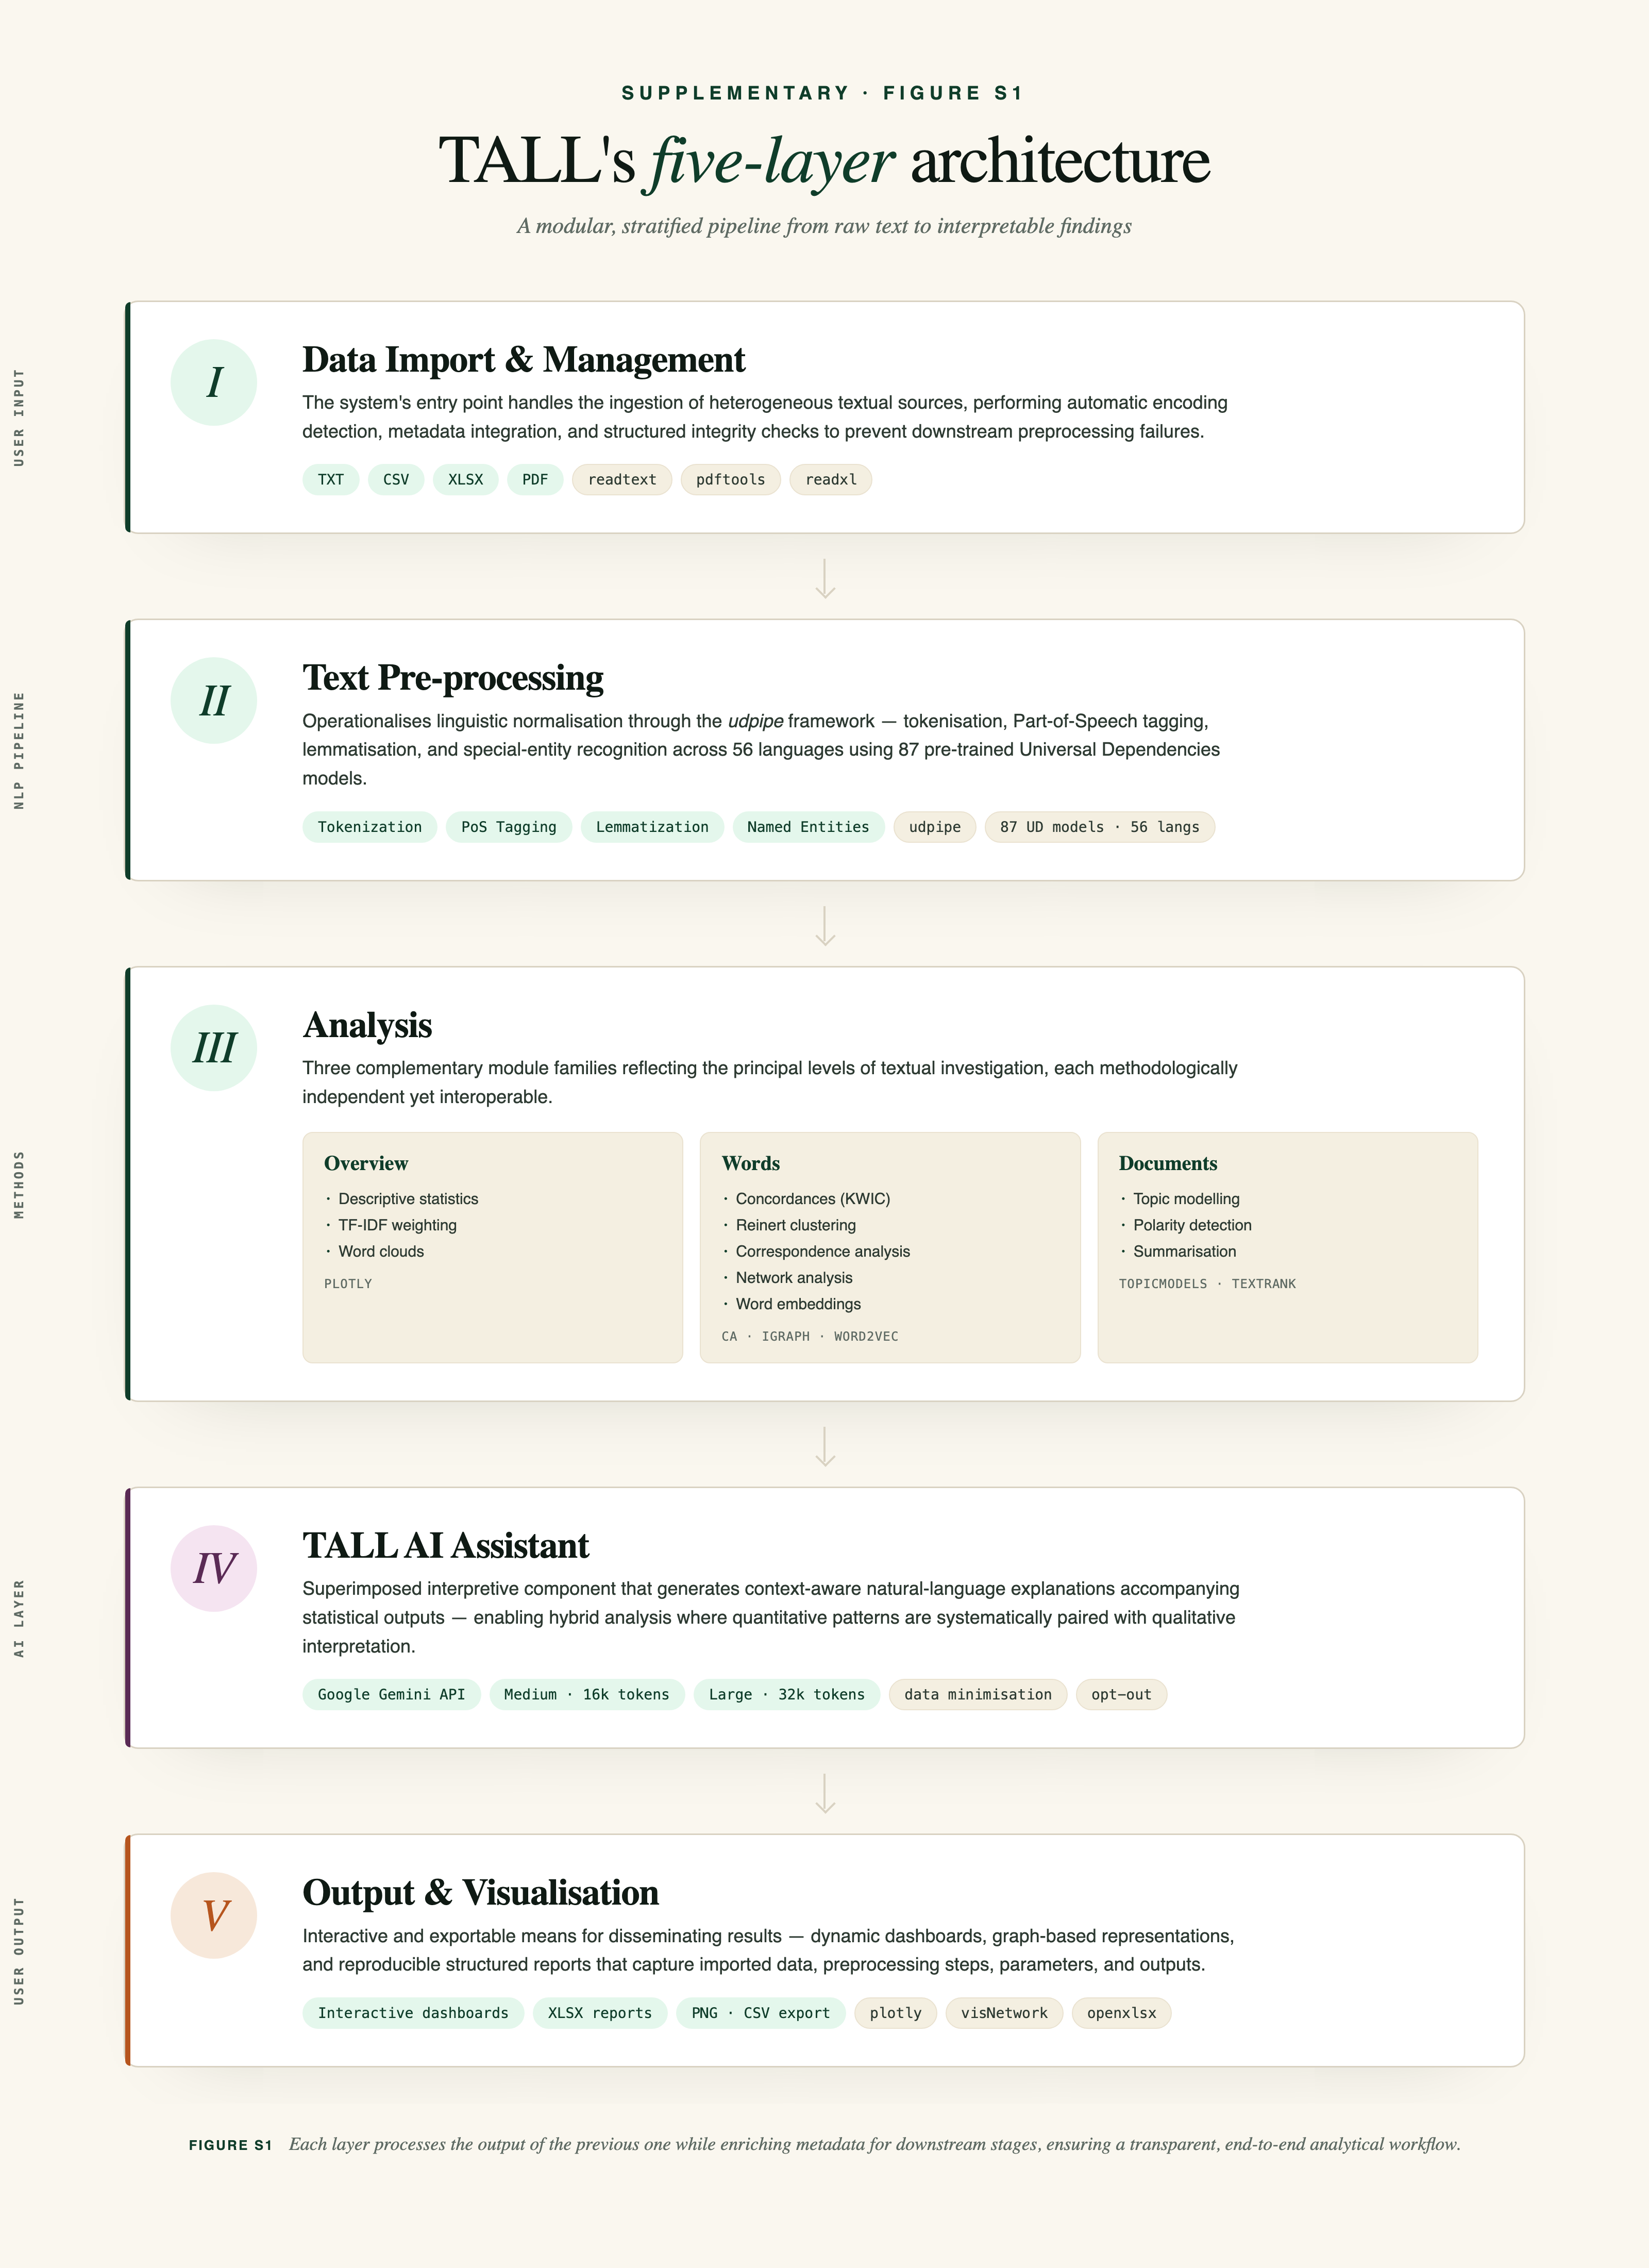
\includegraphics[width=0.85\textwidth]{figure_diagram.png}}
\caption{TALL architecture diagram.}
\label{fig:diagram}
\end{figure}

\section*{D. \quad  Computational Performance Analysis}

To provide practitioners with practical guidance on TALL's computational requirements and scalability characteristics, we conducted comprehensive performance benchmarking across a wide range of corpus sizes. This analysis measures the computational efficiency of TALL's core analytical operations, enabling researchers to make informed decisions about hardware requirements and deployment strategies for their specific use cases.

All benchmarks were executed on a standardized research workstation with the following specifications:

\begin{itemize}
    \item \textbf{Processor:} Apple M4 Pro (14 cores: 10 performance + 4 efficiency, ARM architecture)
    \item \textbf{Memory:} 48 GB unified memory
    \item \textbf{Operating System:} macOS 15.3.0 (Darwin 25.3.0)
    \item \textbf{R Version:} 4.5.2 (2025-10-31)
    \item \textbf{TALL Version:} 0.5.1
\end{itemize}

To ensure reproducibility and linguistic realism, synthetic corpora were generated by sampling sentences with replacement from Herman Melville's \textit{Moby Dick}. We employed a factorial design across 14 configurations, varying document counts (10 to 10,000) and sentences per document (1 to 100), resulting in token counts spanning four orders of magnitude (78 to 5.3M tokens). The 10,000-document/100-sentence setting was excluded due to hardware memory constraints ($>64$ GB RAM required). Seven core operations representing the main approaches of the complete analytical workflow were benchmarked: \textbf{Preprocessing} (Tokenization, lemmatization, and PoS Tagging), \textbf{Multiword Extraction} (Rake approach), \textbf{Keyness Analysis} (reference-based $\chi^2$), \textbf{Topic Modeling} (LDA with 5 topics), \textbf{Word Embeddings} (Word2Vec), \textbf{Network Analysis} (Louvain community detection) and \textbf{Polarity Analysis} (Hu-Liu lexicon scoring). Performance was assessed over 10 iterations per configuration using the \texttt{bench} package \cite{bench25}. We reported median execution times to mitigate the influence of outliers and mean memory allocation to track peak consumption. To ensure reliability, system caches were cleared between runs and background processes were strictly minimized.

Table~S3 presents comprehensive performance metrics across all tested configurations. Figure~\ref{fig:performance_time} and Figure~\ref{fig:performance_memory} visualize execution time and memory consumption as functions of corpus size (measured in total tokens).

\begin{table}[!h]
\centering
\label{tab:tall_performance}
\caption{TALL computational performance benchmarks across different corpus sizes. Values represent median execution time (seconds) and mean peak memory allocation (MB) over 10 iterations for seven core operations. Corpus generated by random sampling with replacement from Herman Melville's \textit{Moby Dick}.}
\centering
\resizebox{\ifdim\width>\linewidth\linewidth\else\width\fi}{!}{
\fontsize{9}{11}\selectfont
\begin{tabular}[t]{lrrrrrrrrrrrrrrr}
\toprule
\multicolumn{2}{c}{ } & \multicolumn{7}{c}{Execution Time (sec)} & \multicolumn{7}{c}{Memory (MB)} \\
\cmidrule(l{3pt}r{3pt}){3-9} \cmidrule(l{3pt}r{3pt}){10-16}
\textbf{Setting} & \textbf{N. Tokens} & \textbf{Pre-proc} & \textbf{Multi} & \textbf{Key} & \textbf{TM} & \textbf{Embed} & \textbf{Net} & \textbf{Polar} & \textbf{Pre-proc} & \textbf{Multi} & \textbf{Key} & \textbf{TM} & \textbf{Embed} & \textbf{Net} & \textbf{Polar}\\
\midrule
10 docs, 1 sent & 78 & 0.53 & 0.01 & 3.15 & 0.00 & 0.00 & 0.02 & 0.01 & 0.1 & 1.1 & 390.4 & 0.5 & 0.1 & 3.4 & 2.7\\
10 docs, 10 sent & 1,103 & 0.60 & 0.01 & 3.88 & 0.01 & 0.01 & 0.03 & 0.01 & 0.3 & 1.6 & 391.7 & 1.0 & 0.3 & 7.2 & 3.6\\
10 docs, 100 sent & 10,436 & 1.31 & 0.04 & 3.81 & 0.05 & 0.02 & 0.05 & 0.04 & 1.8 & 8.0 & 396.3 & 4.4 & 2.5 & 16.1 & 13.4\\
100 docs, 1 sent & 1,155 & 0.62 & 0.01 & 3.42 & 0.01 & 0.01 & 0.03 & 0.02 & 0.2 & 1.6 & 391.8 & 1.1 & 0.3 & 3.0 & 4.1\\
100 docs, 10 sent & 9,920 & 1.15 & 0.04 & 3.37 & 0.06 & 0.02 & 0.05 & 0.05 & 2.0 & 8.0 & 396.3 & 5.5 & 2.5 & 15.8 & 14.1\\
\addlinespace
100 docs, 100 sent & 106,696 & 7.96 & 0.27 & 3.64 & 0.46 & 0.23 & 0.16 & 0.35 & 15.1 & 64.0 & 473.4 & 36.6 & 24.3 & 60.3 & 113.0\\
1000 docs, 1 sent & 11,372 & 0.96 & 0.04 & 3.52 & 0.06 & 0.02 & 0.05 & 0.11 & 2.1 & 8.1 & 396.8 & 6.1 & 2.6 & 12.2 & 18.6\\
1000 docs, 10 sent & 106,213 & 6.94 & 0.25 & 3.60 & 0.53 & 0.22 & 0.16 & 0.58 & 15.2 & 64.0 & 464.4 & 45.6 & 24.5 & 60.9 & 120.9\\
1000 docs, 100 sent & 1,064,577 & 73.21 & 1.70 & 3.73 & 4.79 & 2.33 & 1.20 & 3.76 & 138.2 & 555.3 & 1153.5 & 344.5 & 249.9 & 486.8 & 1115.6\\
5000 docs, 1 sent & 54,460 & 2.79 & 0.15 & 3.92 & 0.29 & 0.12 & 0.11 & 0.60 & 8.2 & 33.6 & 427.8 & 27.0 & 12.7 & 36.8 & 83.9\\
\addlinespace
5000 docs, 10 sent & 532,328 & 32.44 & 0.88 & 4.10 & 2.54 & 1.19 & 0.62 & 2.03 & 70.3 & 284.5 & 766.8 & 219.0 & 125.2 & 252.6 & 595.4\\
5000 docs, 100 sent & 5,331,261 & 398.78 & 7.77 & 5.59 & 23.98 & 11.61 & 5.14 & 16.48 & 678.8 & 2730.2 & 4435.1 & 1669.8 & 1235.5 & 2405.0 & 5585.5\\
10000 docs, 1 sent & 109,237 & 5.56 & 0.24 & 3.83 & 0.58 & 0.24 & 0.17 & 1.11 & 15.2 & 66.8 & 484.8 & 53.7 & 25.9 & 66.9 & 166.8\\
10000 docs, 10 sent & 1,070,462 & 64.06 & 1.65 & 3.76 & 5.48 & 2.40 & 1.16 & 4.32 & 139.3 & 552.6 & 1156.5 & 435.6 & 250.9 & 492.0 & 1192.4\\
\bottomrule
\end{tabular}}
\end{table}

\begin{figure}[htbp]
    \centering
    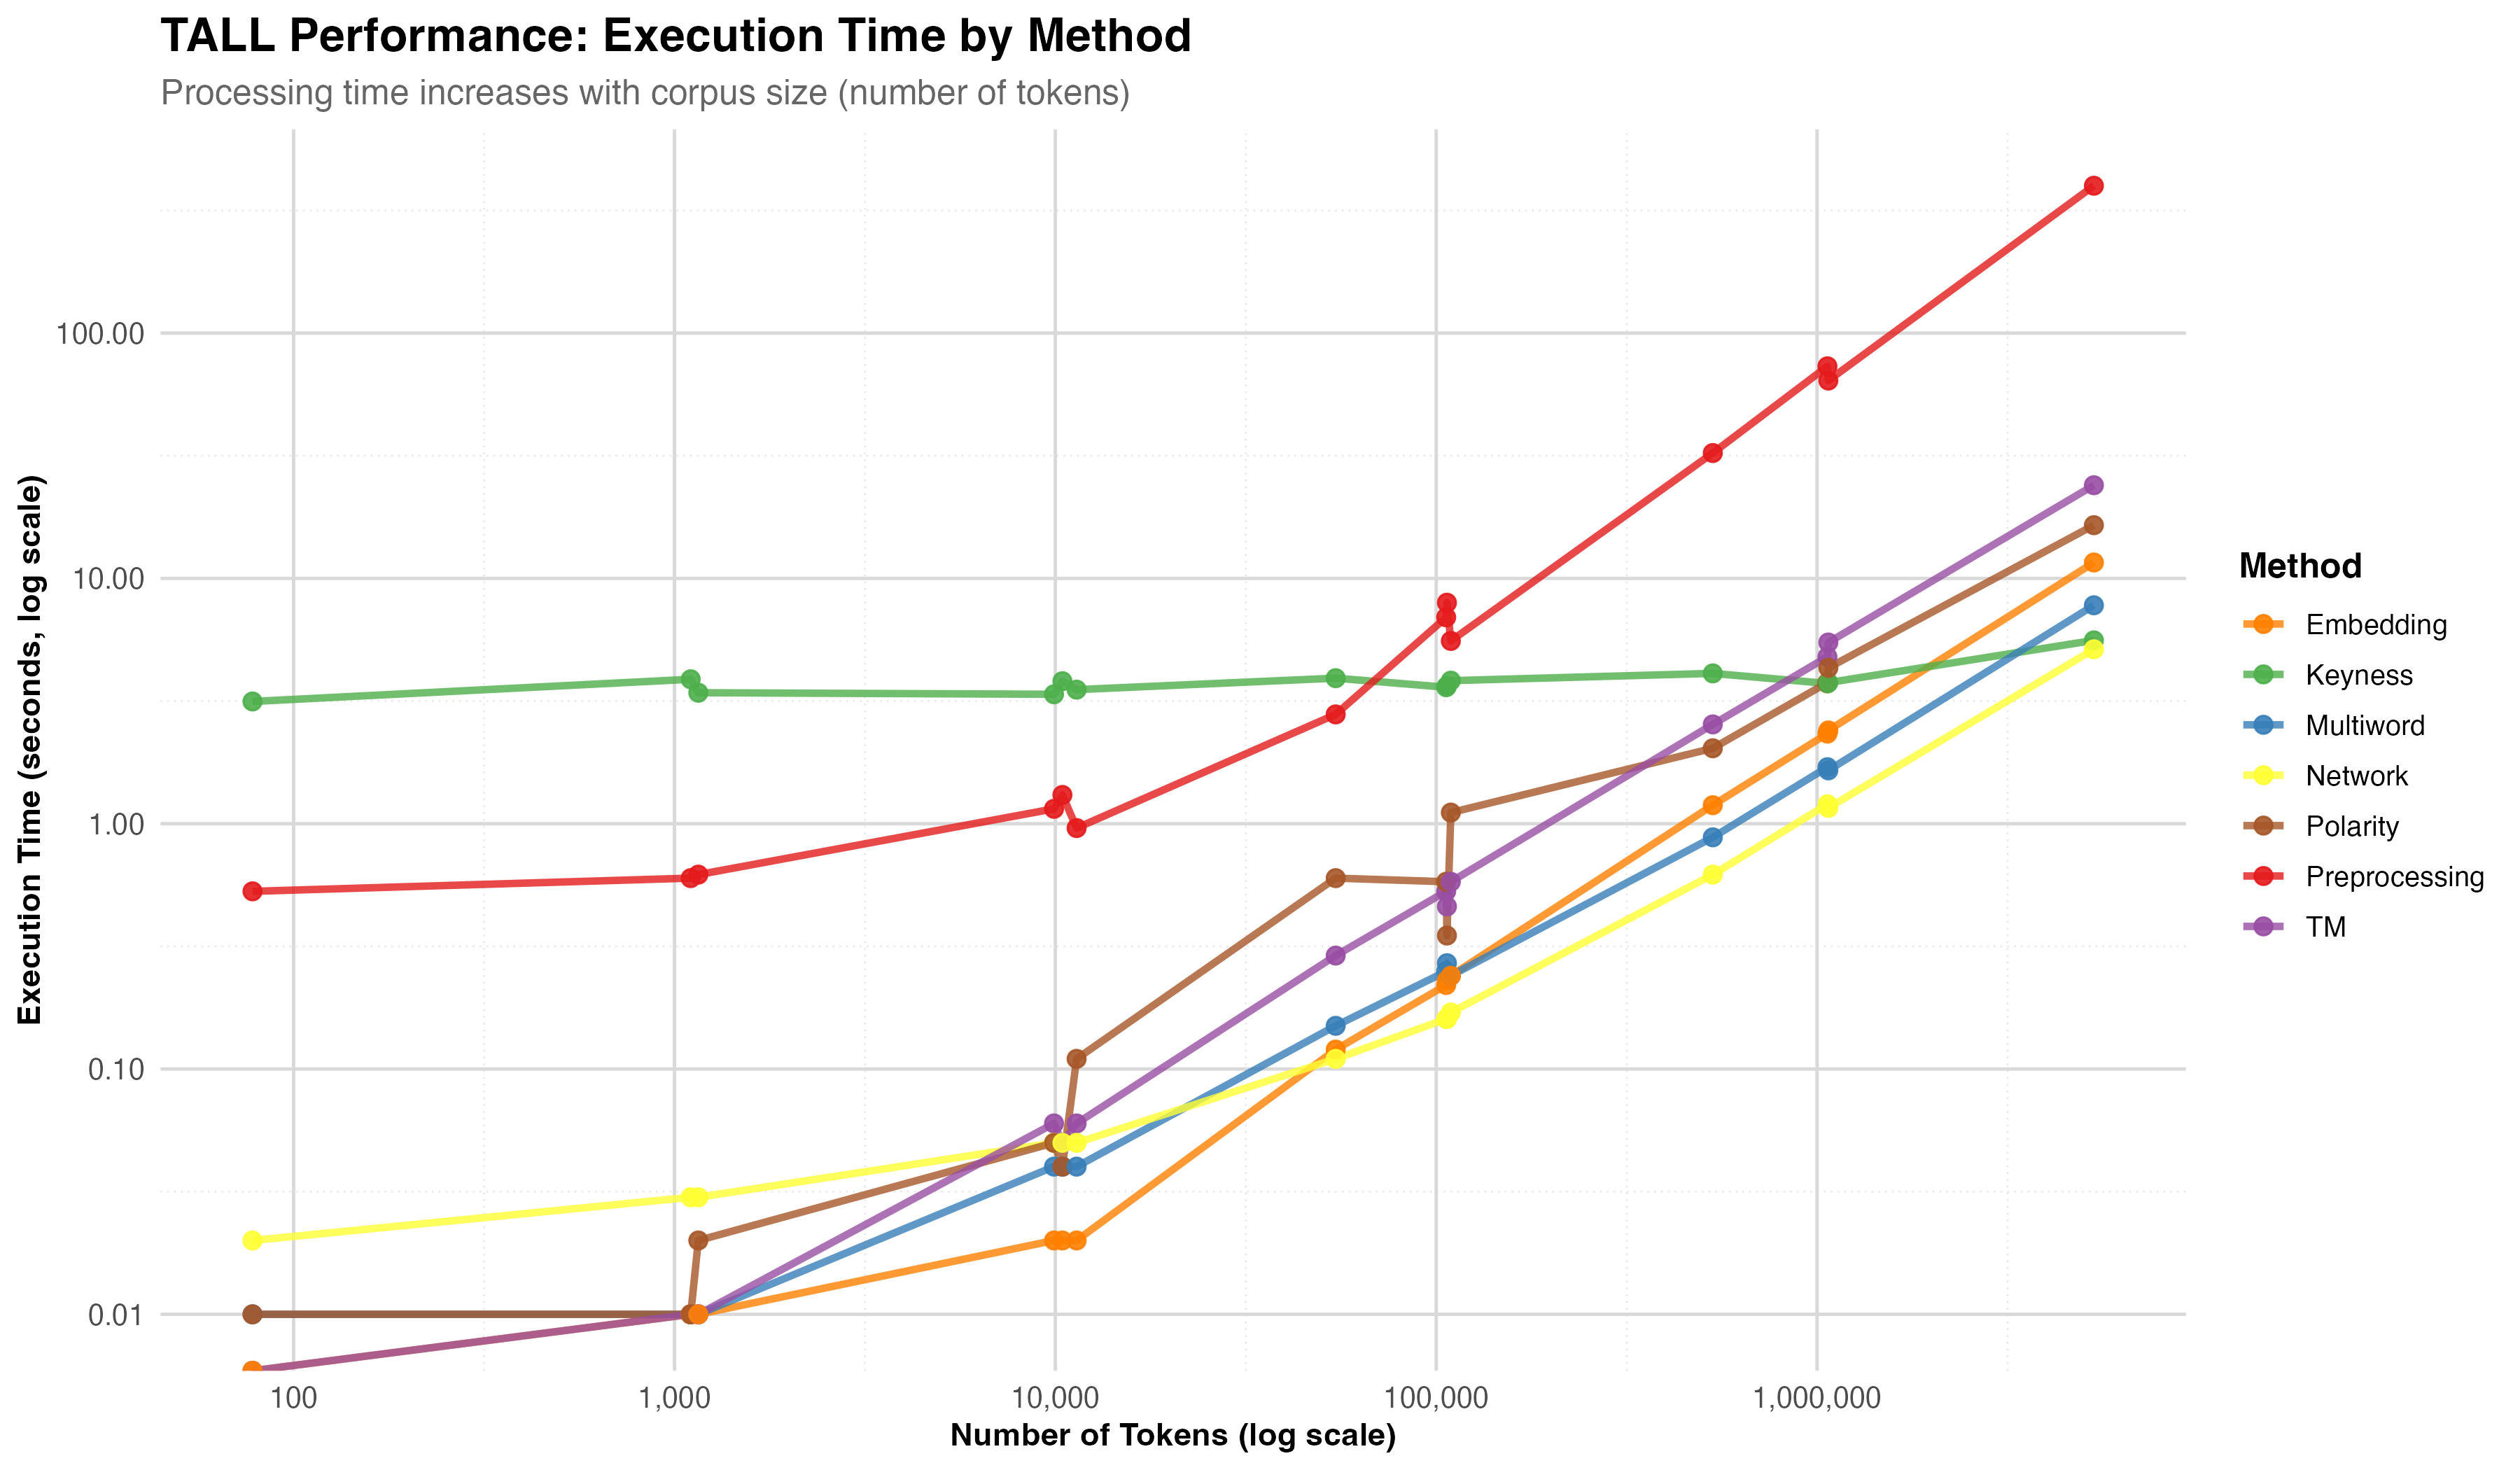
\includegraphics[width=0.9\textwidth]{tall_execution_time_by_tokens.png}
    \caption{TALL execution time for core operations across different corpus sizes. Lines show median execution time over 10 iterations for each corpus configuration, plotted against total token count. Both axes use logarithmic scales.}
    \label{fig:performance_time}
\end{figure}

\begin{figure}[htbp]
    \centering
    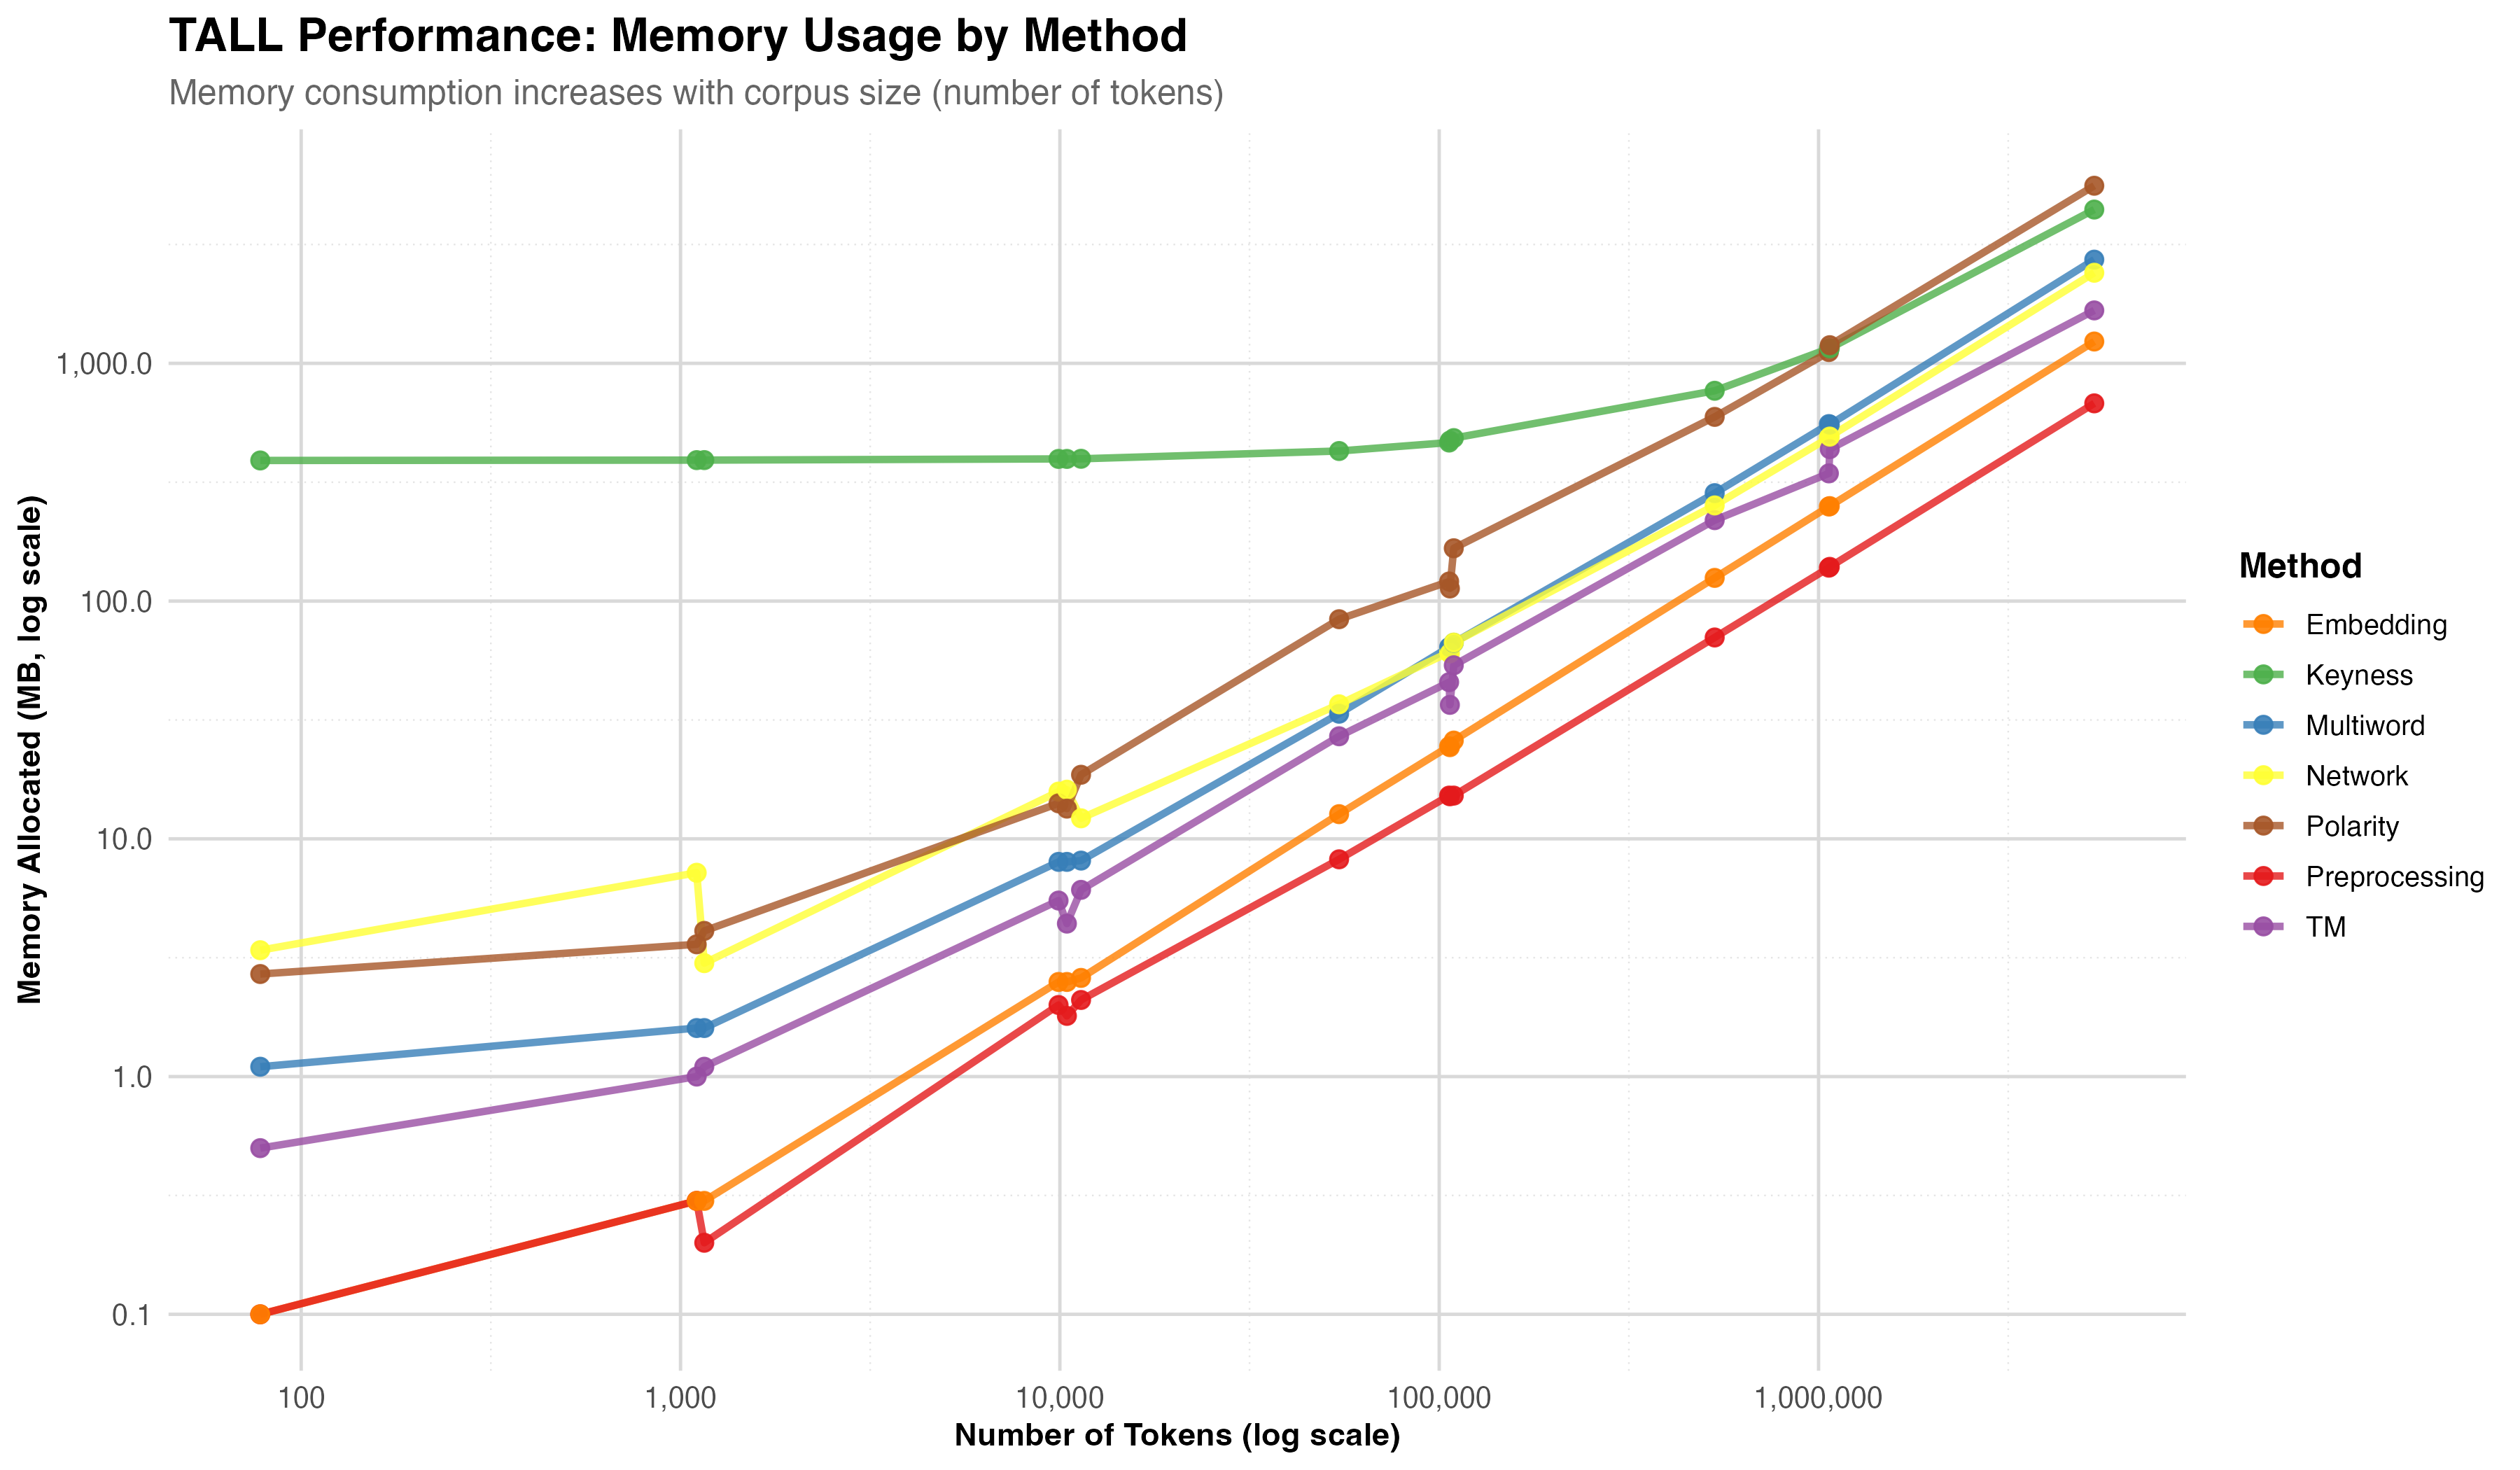
\includegraphics[width=0.9\textwidth]{tall_memory_usage_by_tokens.png}
    \caption{TALL memory usage for core operations across different corpus sizes. Points show mean peak memory allocation over 10 iterations for each corpus configuration, plotted against total token count. Both axes use logarithmic scales.}
    \label{fig:performance_memory}
\end{figure}

Benchmarking results demonstrate that TALL's operations scale efficiently with corpus size. \textbf{Preprocessing} exhibits linear scaling ($O(n)$), processing approximately 14,500 tokens/sec on Apple M4 Pro hardware, with stable performance for corpora exceeding 1,000 tokens. \textbf{Multiword Extraction}, powered by Rcpp-optimized engines, proved remarkably fast (max 7.77s for 5.3M tokens), while \textbf{Word Embeddings} and \textbf{Topic Modeling} showed efficient parallelization and modest computational costs, making them accessible without high-performance computing infrastructure. In contrast, \textbf{Keyness Analysis} and \textbf{Polarity Analysis} are driven primarily by reference vocabulary size rather than raw token counts. While execution times for Keyness remained stable (3.15--5.59s), memory consumption scaled significantly (up to 4.4GB), marking it as the most memory-intensive operation for large datasets. \textbf{Network Analysis} similarly maintained efficiency through TALL's vocabulary reduction strategies.

Memory patterns indicate that TALL is highly versatile: small to medium corpora ($<10^5$ tokens) operate within 1--2GB RAM, suitable for standard laptops. Large corpora ($10^5$--$10^6$ tokens) require approximately 5GB, while very large datasets ($>10^6$ tokens) can exceed 10GB during vocabulary-intensive tasks, suggesting a transition from desktop workstations to institutional servers for optimal performance at scale.

The analysis conducted on realistically generated literary corpora indicates that TALL achieves a favourable balance between usability and computational efficiency. The empirical results show that the preprocessing stage scales approximately linearly with corpus size, whereas performance-critical components -- such as keyness computation and multi-word extraction -- benefit from \texttt{Rcpp}-based implementations that maintain acceptable execution times as memory requirements increase with vocabulary size. Importantly, the observed performance profiles demonstrate that analytically demanding procedures, including topic modelling and word embedding estimation, can be applied to corpora of approximately one million tokens on standard research hardware (approximately 16 GB of RAM) without requiring specialised high-performance computing resources. At the same time, the architecture remains compatible with server-based deployment, enabling the analysis of substantially larger corpora in institutional settings.

%Taken together, these findings provide empirical support for TALL’s design rationale, namely the provision of advanced NLP and text mining capabilities within a computationally predictable and accessible framework. By reporting quantitative benchmarks for runtime and memory consumption across representative analytical tasks, the study enables researchers to assess hardware requirements and workflow feasibility a priori, thereby positioning TALL as an effective intermediary between established computational methods and interactive, reproducible text analysis environments.

\section*{E. \quad Adoption and usage: CRAN downloads}

Fig.~\ref{fig:cran_downloads} presents the cumulative monthly downloads of the \texttt{tall} package from the \textit{Comprehensive R Archive Network} (CRAN) over the period spanning its initial public release in February 2025 through November 2025 (source: \textit{CRANlogs}, \url{https://cranlogs.r-pkg.org}). The curve displays a consistent upward trajectory, with cumulative counts rising from fewer than 300 downloads in the release month to more than 4{,}000 by the end of November. The figure highlights a marked acceleration between April and June~2025, corresponding to an early phase of adoption in which the user base expands rapidly, followed by a period of sustained, near-linear growth from midsummer onwards. The progression suggests that the app achieved stable uptake beyond its initial launch period, with each successive month contributing a substantial increase in total installations. This cumulative pattern provides empirical evidence of the package’s diffusion within the \texttt{R} ecosystem, illustrating both its early visibility and its continued integration into analytical workflows over the months.

\begin{figure}[!ht]
\centering
\fbox{\includegraphics[width=0.95\textwidth]{TALL_download_nov2025.png}}
\caption{Cumulative daily downloads of \texttt{tall} from CRAN (February -- November 2025).}
\label{fig:cran_downloads}
\end{figure}

\section*{F. \quad A step-by-step example}

This section provides a practical demonstration of the TALL application through a step-by-step example based on a publicly available dataset of \textit{US Airline Tweets} \cite{fig15}. This step-by-step workflow demonstrates TALL's capacity to support comprehensive text analysis without requiring programming expertise. By integrating preprocessing, visualization, and AI-assisted interpretation within a single platform, TALL enables researchers to conduct reproducible and transparent analyses of complex textual data. The US Airline Tweets example illustrates the platform's utility for social media analytics, sentiment detection, and customer feedback analysis, applications relevant across commercial, academic, and policy domains.

\subsection*{Data import and AI-Assisted context}
The US Airline Tweets dataset is included as a built-in example in TALL, providing immediate access without requiring external data loading. Upon importing the dataset, the list of texts is displayed, and users can either view the full content of a specific document or remove it from the list using the \textit{View} and \textit{Remove} buttons, respectively. Additionally, the TALL AI assistant interface is automatically populated with a contextual description of the data (Fig.~\ref{fig:import}). This preconfigured prompt ensures that the AI maintains full awareness of the dataset's characteristics throughout the analytical workflow, enabling context-aware interpretations and recommendations at each stage. This integration exemplifies TALL's hybrid approach to text analysis, combining algorithmic processing with AI-assisted interpretation.

\vspace{\baselineskip}
\noindent\textbf{Key features at this stage:}
\begin{itemize}
    \item Automatic dataset recognition and metadata loading
    \item Pre-populated AI context for enhanced interpretability
    \item Interactive prompt customization options
\end{itemize}

\begin{figure}[!ht]
\centering
\fbox{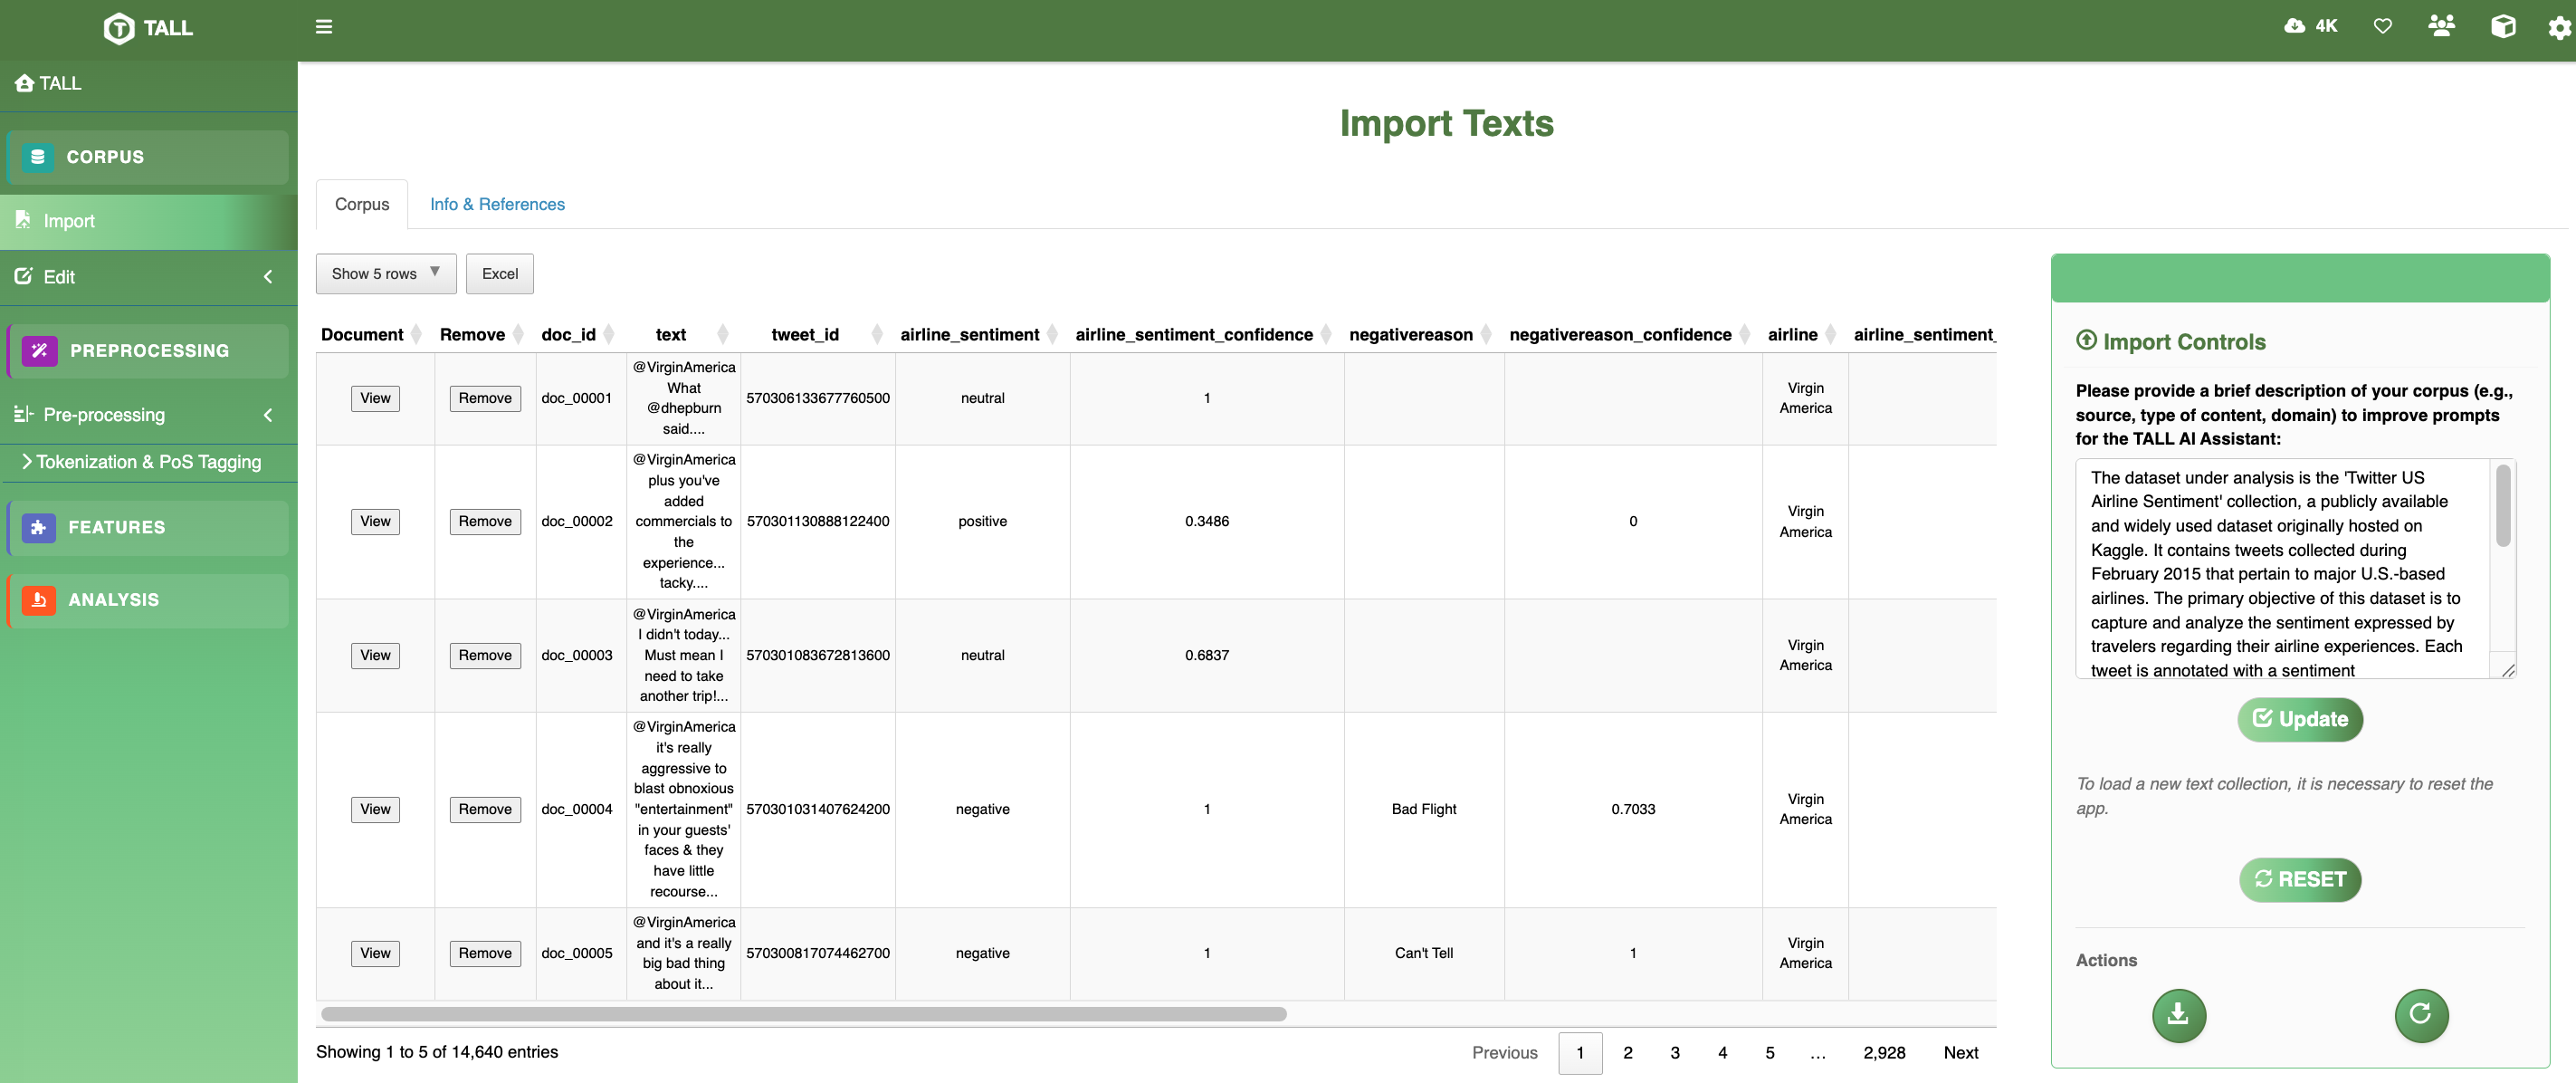
\includegraphics[width=0.85\textwidth]{fig1_import.png}}
\caption{TALL workflow and main components.}
\label{fig:import}
\end{figure}

\subsection*{Tokenization and PoS tagging}
The pre-processing workflow begins with language selection and model specification. For this \textit{corpus}, English is selected as the source language, and the pre-trained EN \textsf{GUM} model \cite{zel17, ari25} is employed. This model offers high accuracy and is specifically trained on diverse text types, including web-based content suitable for social media analysis. During tokenization, each row in the resulting dataframe corresponds to a single token, followed by its lemma and Part-of-Speech (PoS) tag. Users can specify whether subsequent analyses should operate on tokens or lemmas through the unit selection interface, with the current choice displayed prominently in the upper-right banner (Fig.~\ref{fig:tokenization}). This flexibility allows researchers to adapt their analytical focus based on research objectives, whether prioritizing morphological variation (tokens) or semantic grouping (lemmas).

\vspace{\baselineskip}
\noindent\textbf{Pre-processing specifications:}
\begin{itemize}
    \item Language model: Universal Dependencies \textsf{GUM}
    \item Unit of analysis: Lemma (selected for this workflow)
    \item Output: Annotated token dataframe with lemma and PoS information
\end{itemize}

\begin{figure}[!ht]
    \centering
    \fbox{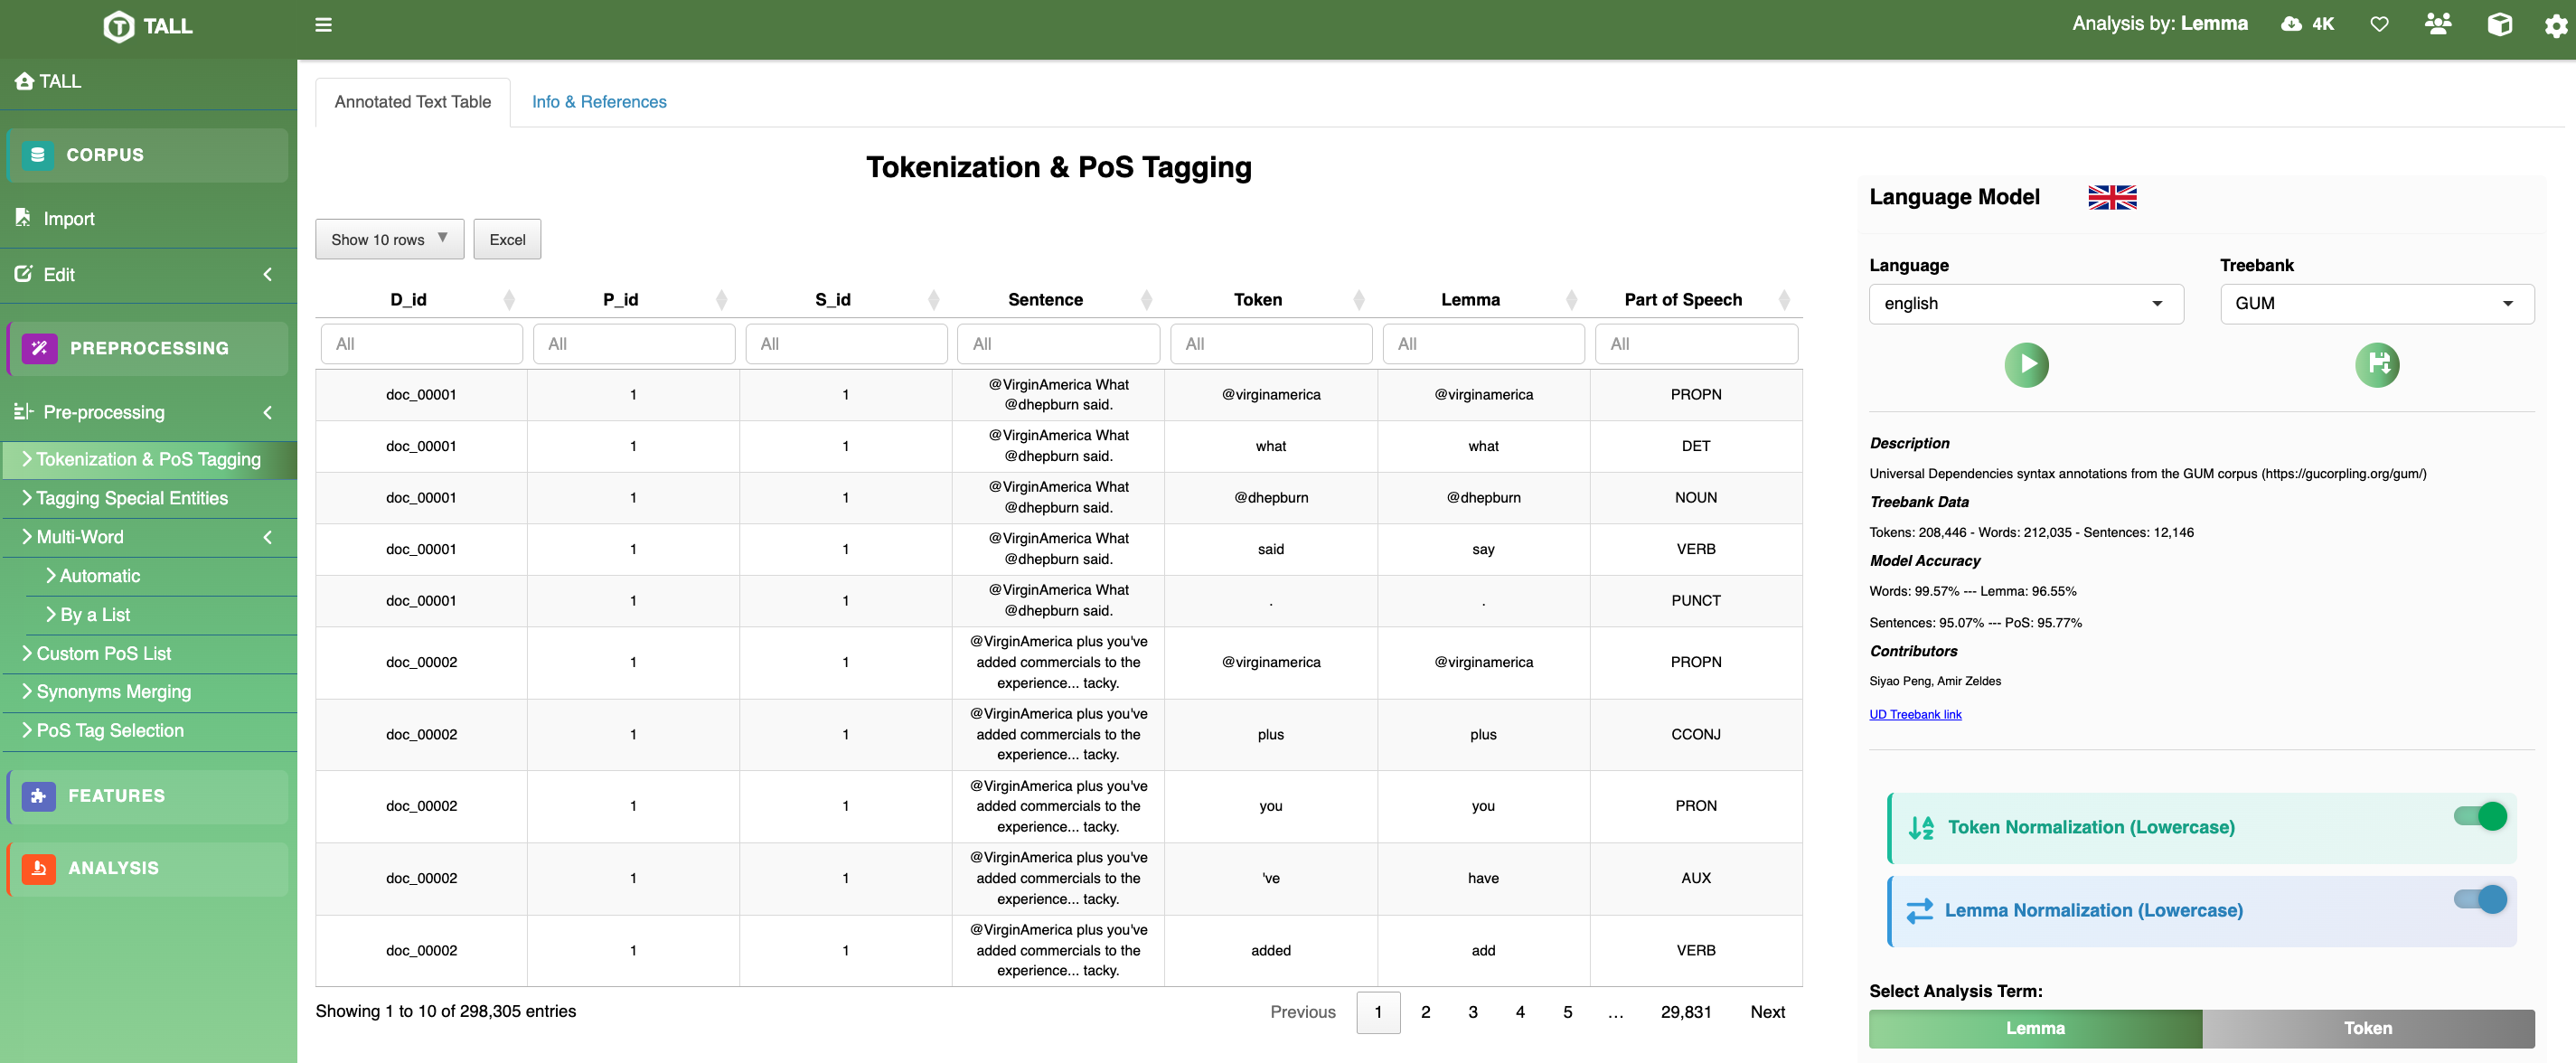
\includegraphics[width=0.85\textwidth]{fig2_tokenization.png}}
    \caption{Tokenization and PoS Tagging.}
    \label{fig:tokenization}
\end{figure}

\subsection*{Special entities' recognition}
Typically, social media texts are characterized by distinctive linguistic features, including emojis, hashtags, and user mentions. TALL allows the identification of these elements as special entities, providing dedicated tools for their extraction and analysis (Fig.~\ref{fig:entities}). Among the different special entities, in the US Airline Tweets \textit{corpus} TALL detected 127 unique emojis, 1,990 unique hashtags (\textsf{HASH}), and 930 user mentions (\textsf{MENTION}). The distribution of the top 10 hashtags is visualized through frequency plots, revealing the most salient issues and keywords within the dataset. Once identified, special entities are automatically tagged in the dataframe, with entity labels replacing the original PoS (Fig.~\ref{fig:entities}). This tagging process enables their inclusion in downstream analyses, either as standalone elements or in combination with standard lexical units.

\vspace{\baselineskip}
\noindent\textbf{Entity recognition outcomes:}
\begin{itemize}
    \item Systematic identification of platform-specific features
    \item Frequency-based ranking and visualization
    \item Integration into the analytical dataframe for unified processing
\end{itemize}

\begin{figure}[!ht]
    \centering
   \fbox{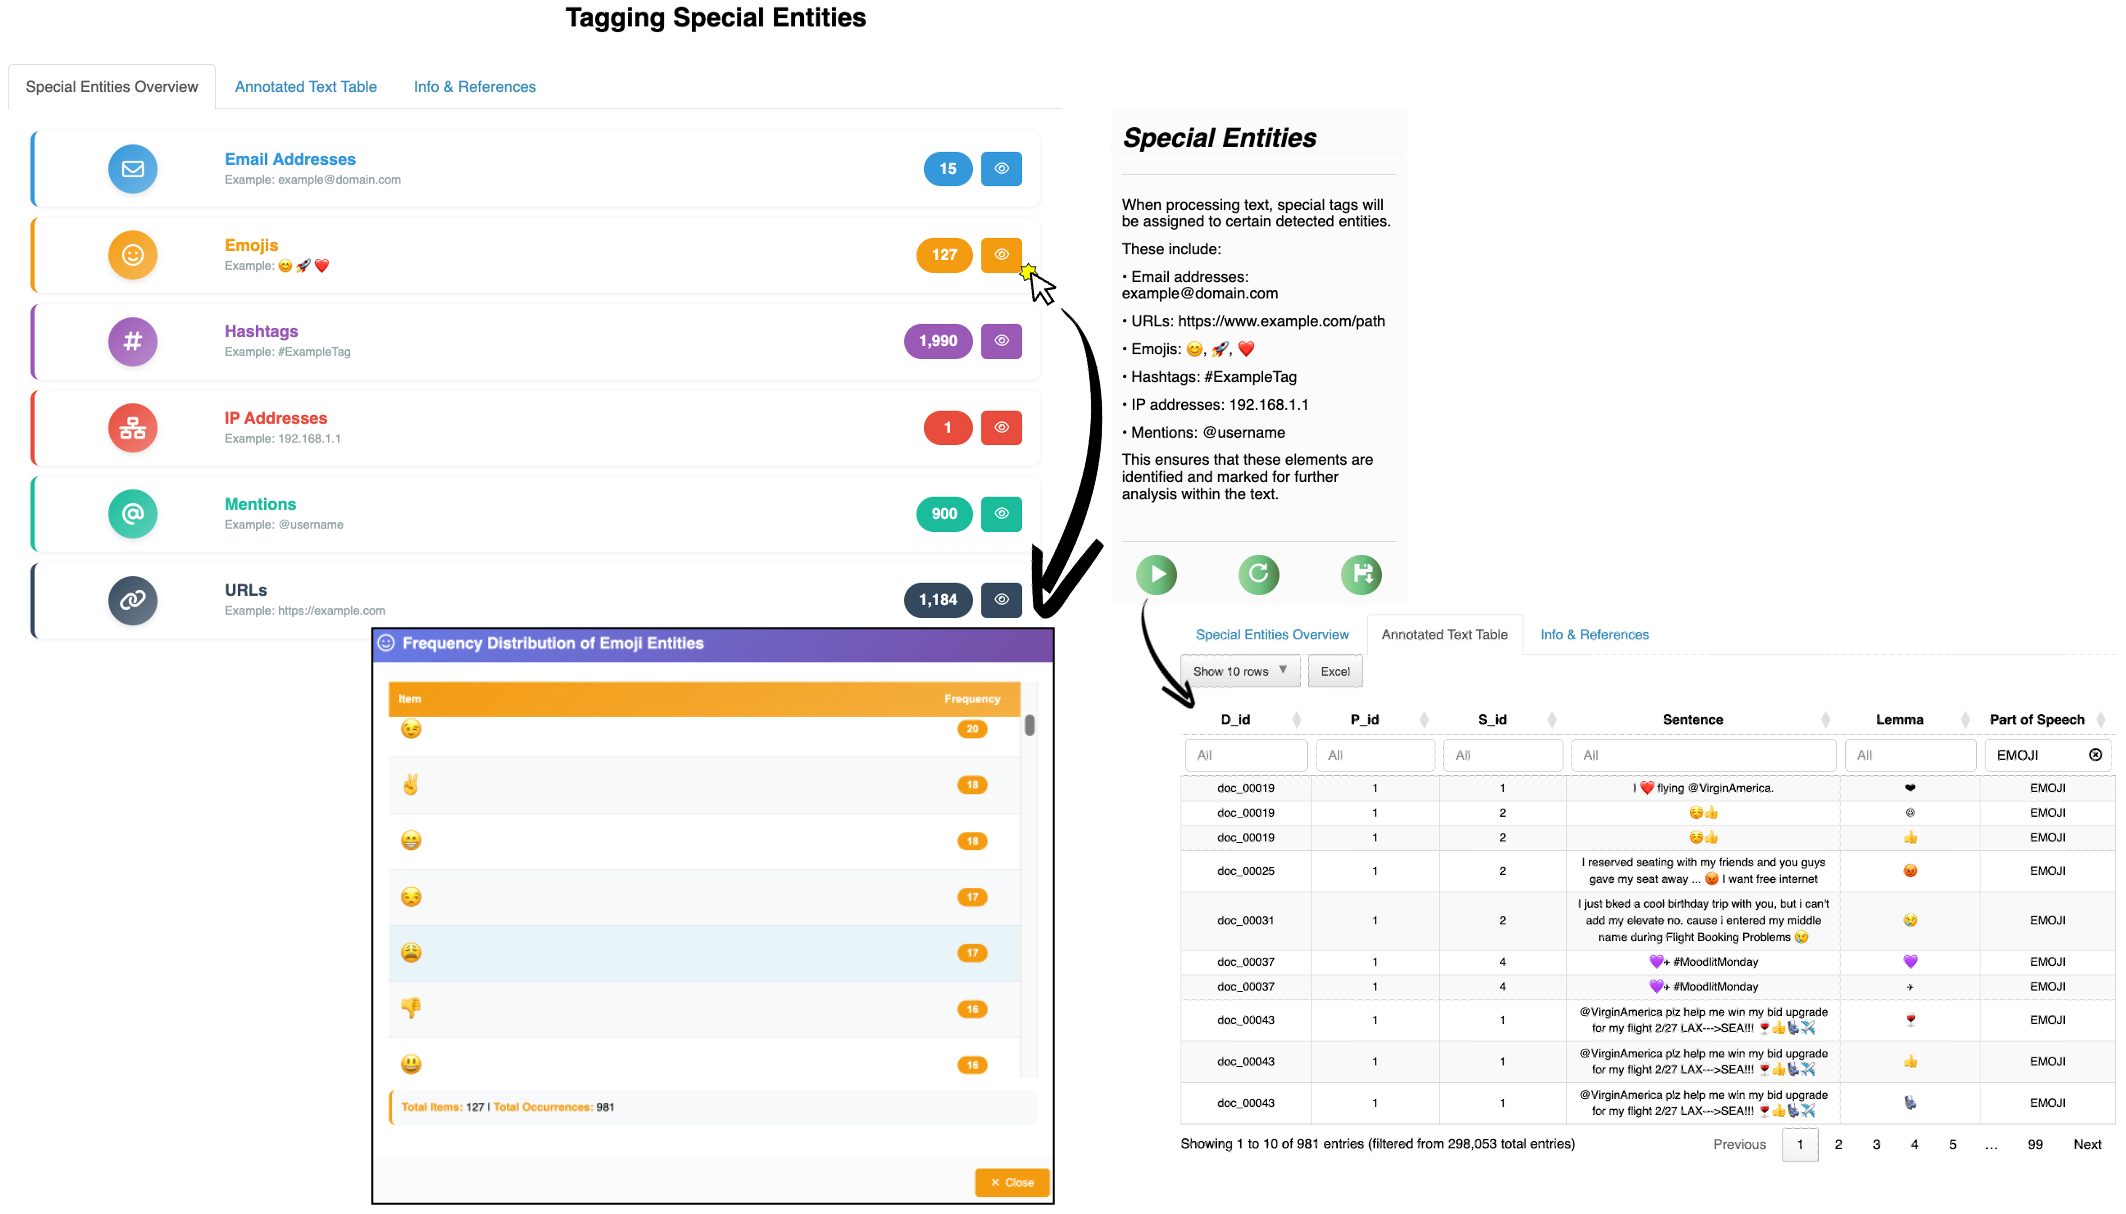
\includegraphics[width=0.85\textwidth]{fig3_entities.png}}
    \caption{Special entities recognition and annotated text.}
    \label{fig:entities}
\end{figure}

\begin{figure}[!ht]
    \centering
    \fbox{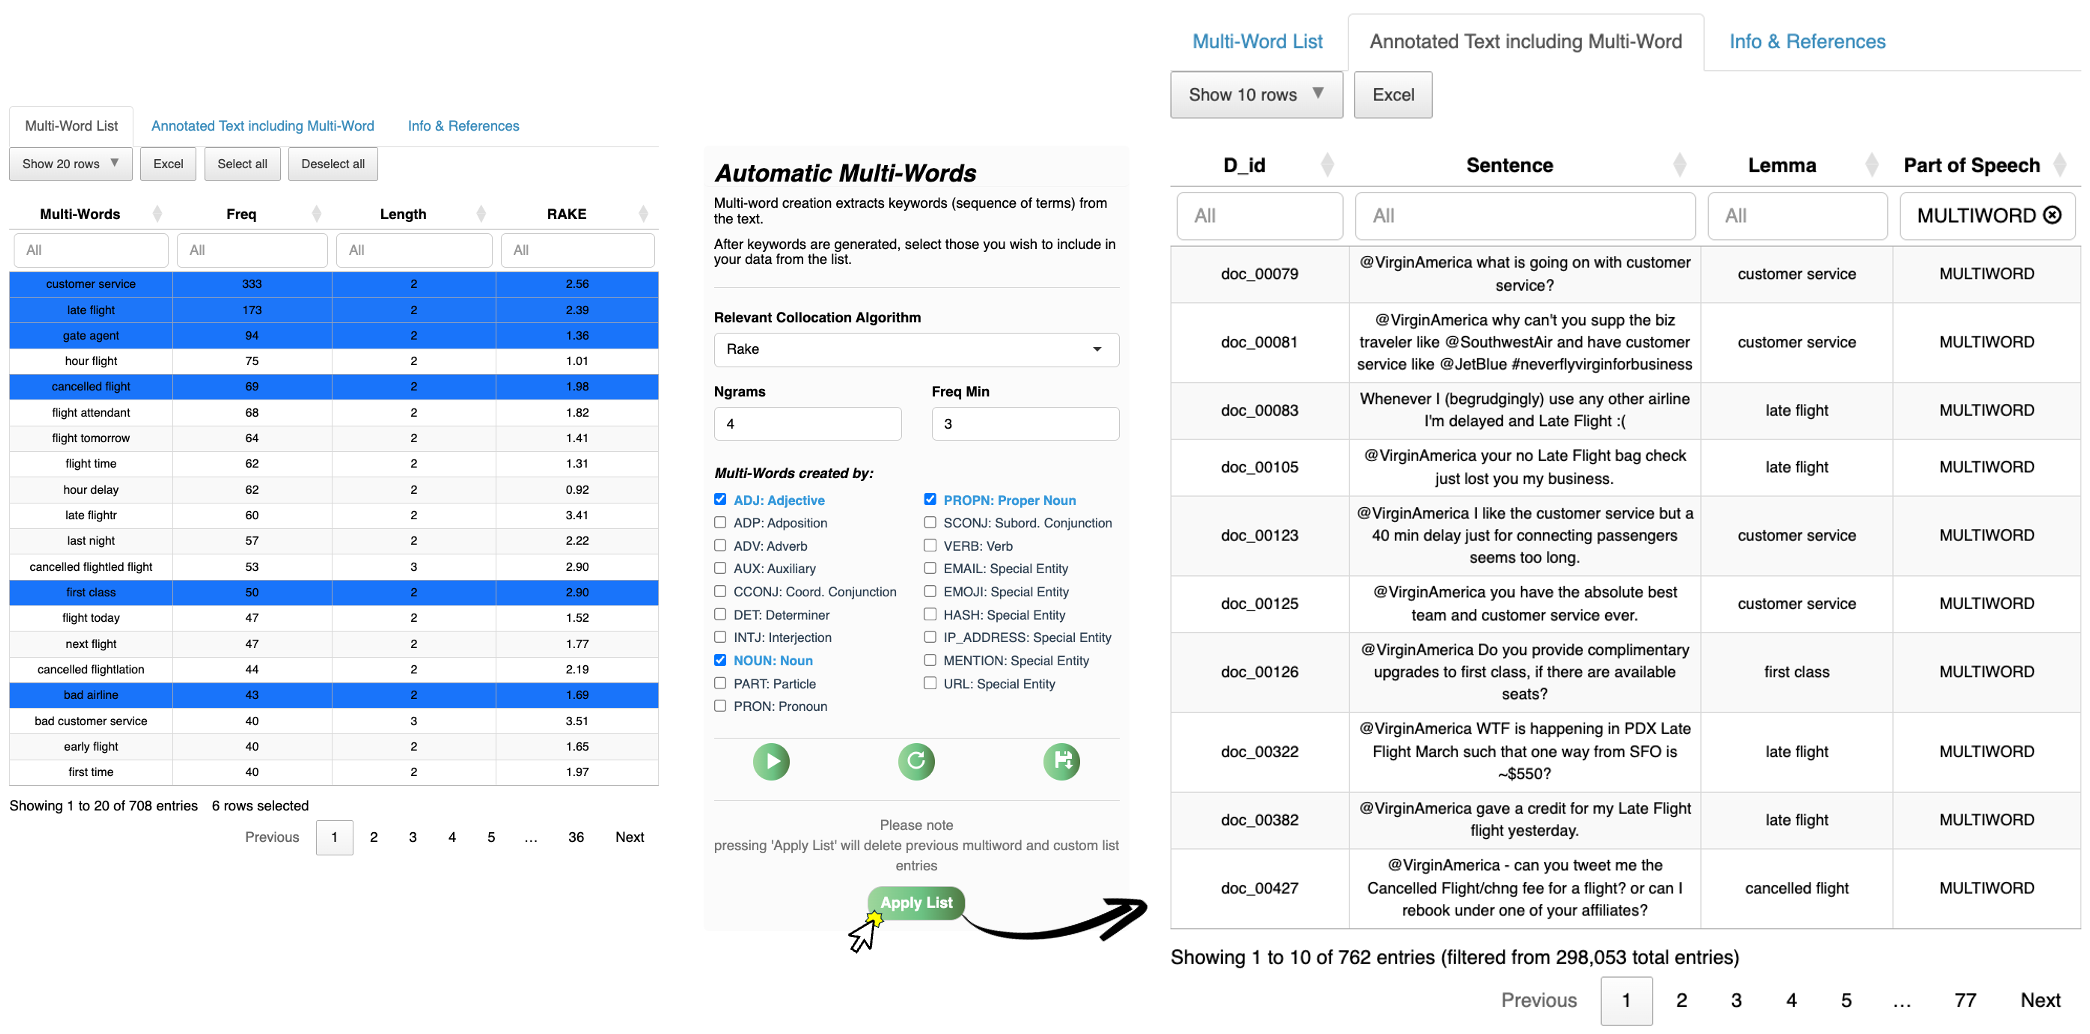
\includegraphics[width=0.85\textwidth]{fig4_multiword.png}}
    \caption{Multi-word creation and candidates' selection.}
    \label{fig:multiword}
\end{figure}

\subsection*{Multi-words' detection and selection}
To capture semantically coherent phrases that function as single conceptual units, TALL provides automated multi-word expression creation. Users can generate multi-words through algorithm-driven identification or by uploading custom phrase lists. For algorithmic extraction, the Rapid Automatic Keyword Extraction (RAKE) algorithm \cite{ros10} is employed, configured with the following parameters:

\begin{enumerate}
    \item Maximum n-gram length: User-specified (e.g., 2--3 tokens)
    \item Minimum frequency threshold: Set based on \textit{corpus} size
    \item PoS filter: Selection of eligible PoS for multi-word construction
\end{enumerate} 

\noindent In the example, the multi-word generation process successfully identified semantically meaningful collocations such as ``customer service'', ``late flight'' and ``flight attendant''. These terms, ranked by frequency, are presented in an interface that allows users to manually select retained candidates. Selected multi-words can be tagged in the main dataframe and treated as single entries in the analyses, preserving their compositional meaning (Fig.~\ref{fig:multiword}).

\vspace{\baselineskip}
\noindent\textbf{Multi-word creation workflow:}
\begin{itemize}
    \item Algorithmic collocation detection via RAKE
    \item Frequency-based ranking and manual curation
    \item Integration into the analytical vocabulary via the \textit{Apply List} function
\end{itemize}

\subsection*{Part-of-Speech selection}
Before proceeding to word-level and document-level analyses, users must specify which lexical categories to include through the PoS Tag Selection menu. The interface presents a comprehensive list of standard POS categories (e.g., nouns, verbs, and adjectives), which are automatically supplemented by custom categories generated in previous steps. Specifically, special entities (emojis, hashtags, mentions) and multi-word appear as selectable categories alongside traditional tags (Fig.~\ref{fig:pos}). This unified selection mechanism ensures that all relevant linguistic units, both conventional and domain-specific, can be incorporated into the analysis. In this example workflow, the following categories were retained:
\begin{enumerate}
    \item Nouns (\textsf{NOUN})
    \item Proper nouns (\textsf{PROPN})
    \item Adjectives (\textsf{ADJ})
    \item Hashtags (\textsf{HASH})
    \item Multi-words (\textsf{MULTIWORD})
\end{enumerate}

\begin{figure}[!ht]
    \centering
    \fbox{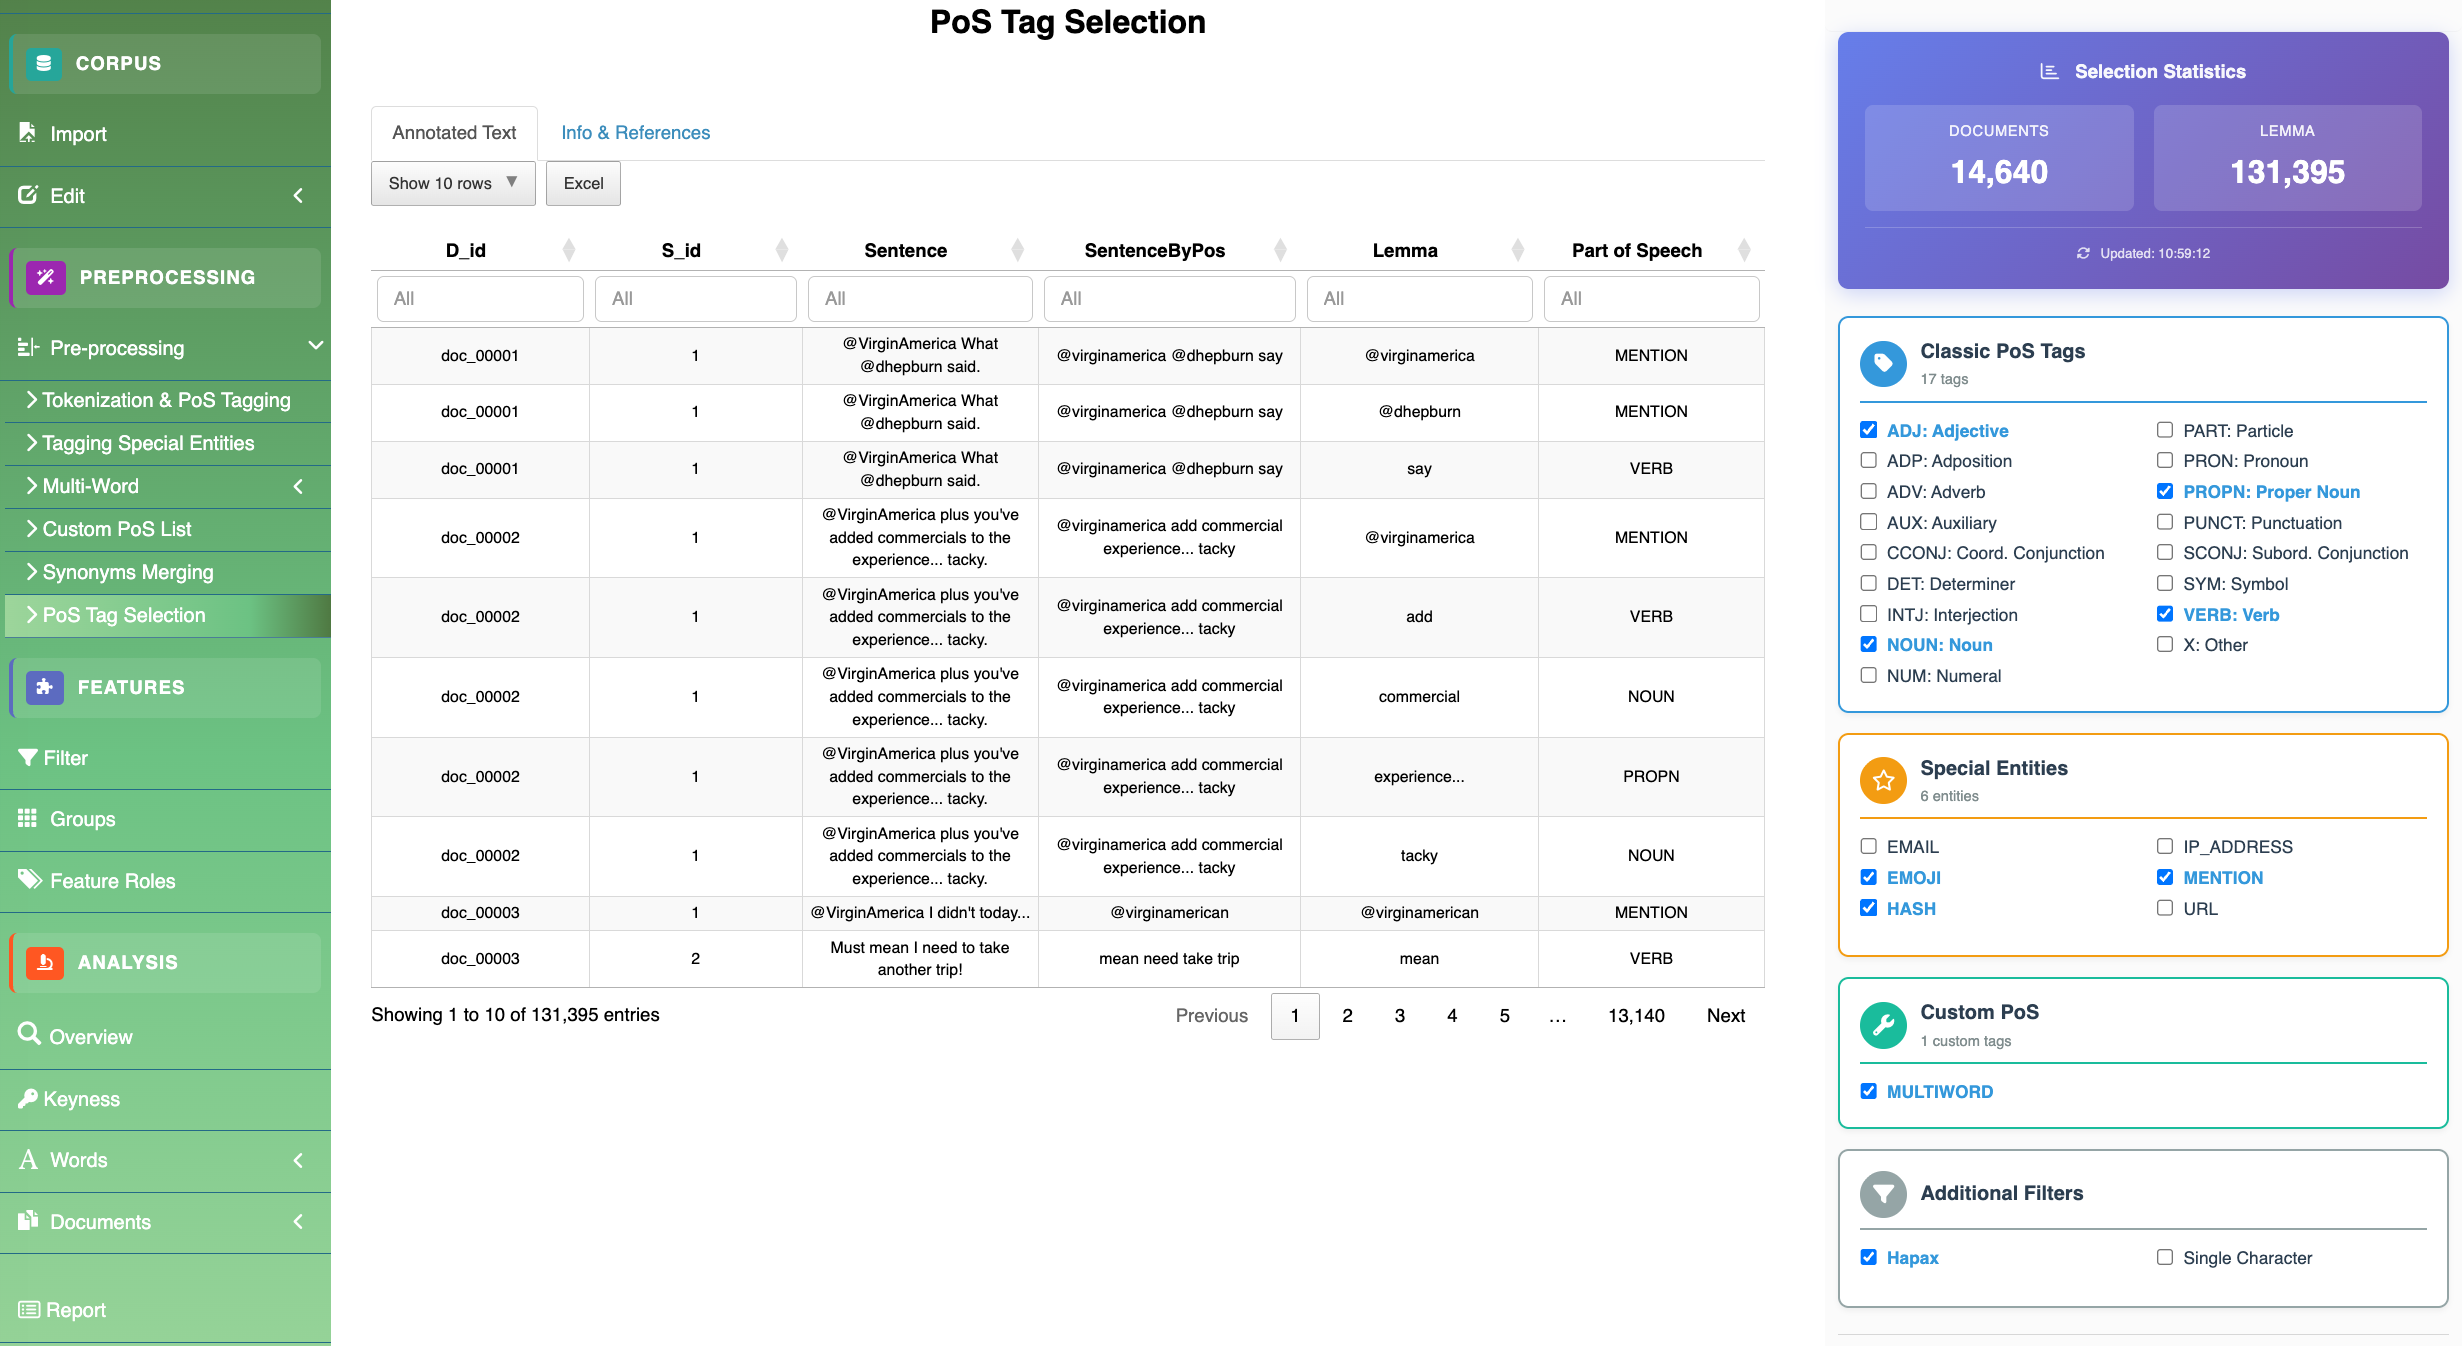
\includegraphics[width=0.85\textwidth]{fig5_pos.png}}
    \caption{PoS Tag selection.}
    \label{fig:pos}
\end{figure}

\subsection*{\textit{Corpus} overview and descriptive statistics}
The Overview module provides a comprehensive descriptive characterization of the corpus, including lexical measures, frequency distributions, and basic statistical summaries. This initial exploration offers essential context for interpreting subsequent analyses and identifying potential research directions. In addition to quantitative outputs, the TALL AI assistant generates natural-language summaries that highlight key patterns and suggest appropriate analytical strategies. For the US Airline Tweets dataset, the AI commentary emphasized the prevalence of service-related terminology and recommended two specific analyses:

\begin{enumerate}
    \item \textbf{Word-in-Context Analysis}: to examine the co-textual usage patterns of specific terms and hashtags
    \item \textbf{Polarity Detection}: to expplore sentiment distributions and identify lexical markers of customer satisfaction and dissatisfaction
\end{enumerate}

\noindent These recommendations guided the subsequent analytical steps, demonstrating the platform's capacity to support both exploratory and hypothesis-driven research (Fig.~\ref{fig:overview}).

\begin{figure}[!ht]
    \centering
    \fbox{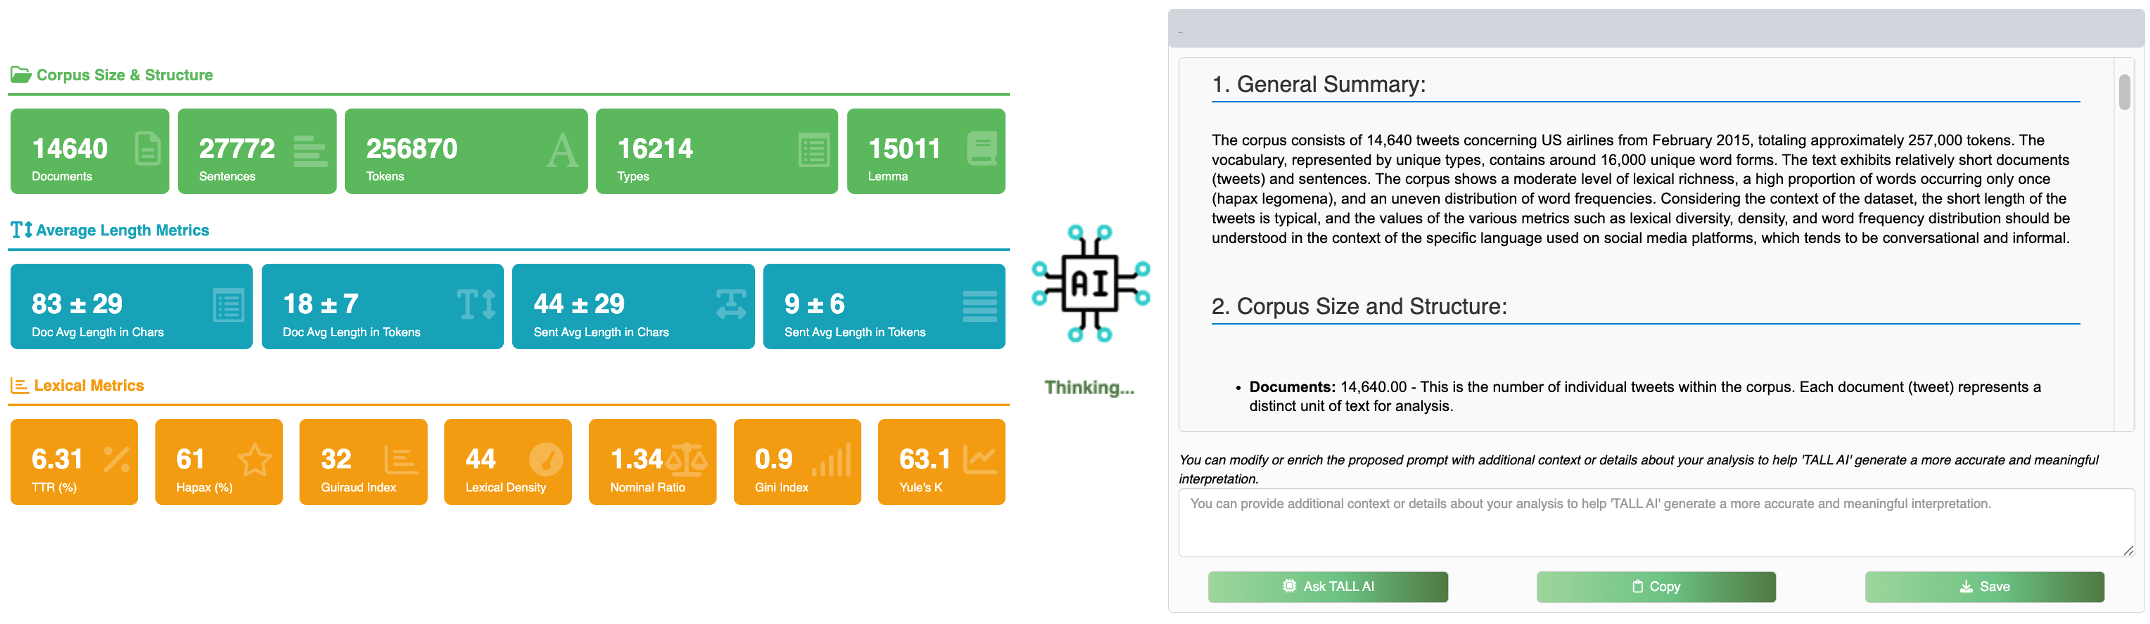
\includegraphics[width=0.85\textwidth]{fig6_overview.png}}
    \caption{Overview and selected TALL AI-based interpretations of key statistics.}
    \label{fig:overview}
\end{figure}

\begin{figure}[!ht]
    \centering
    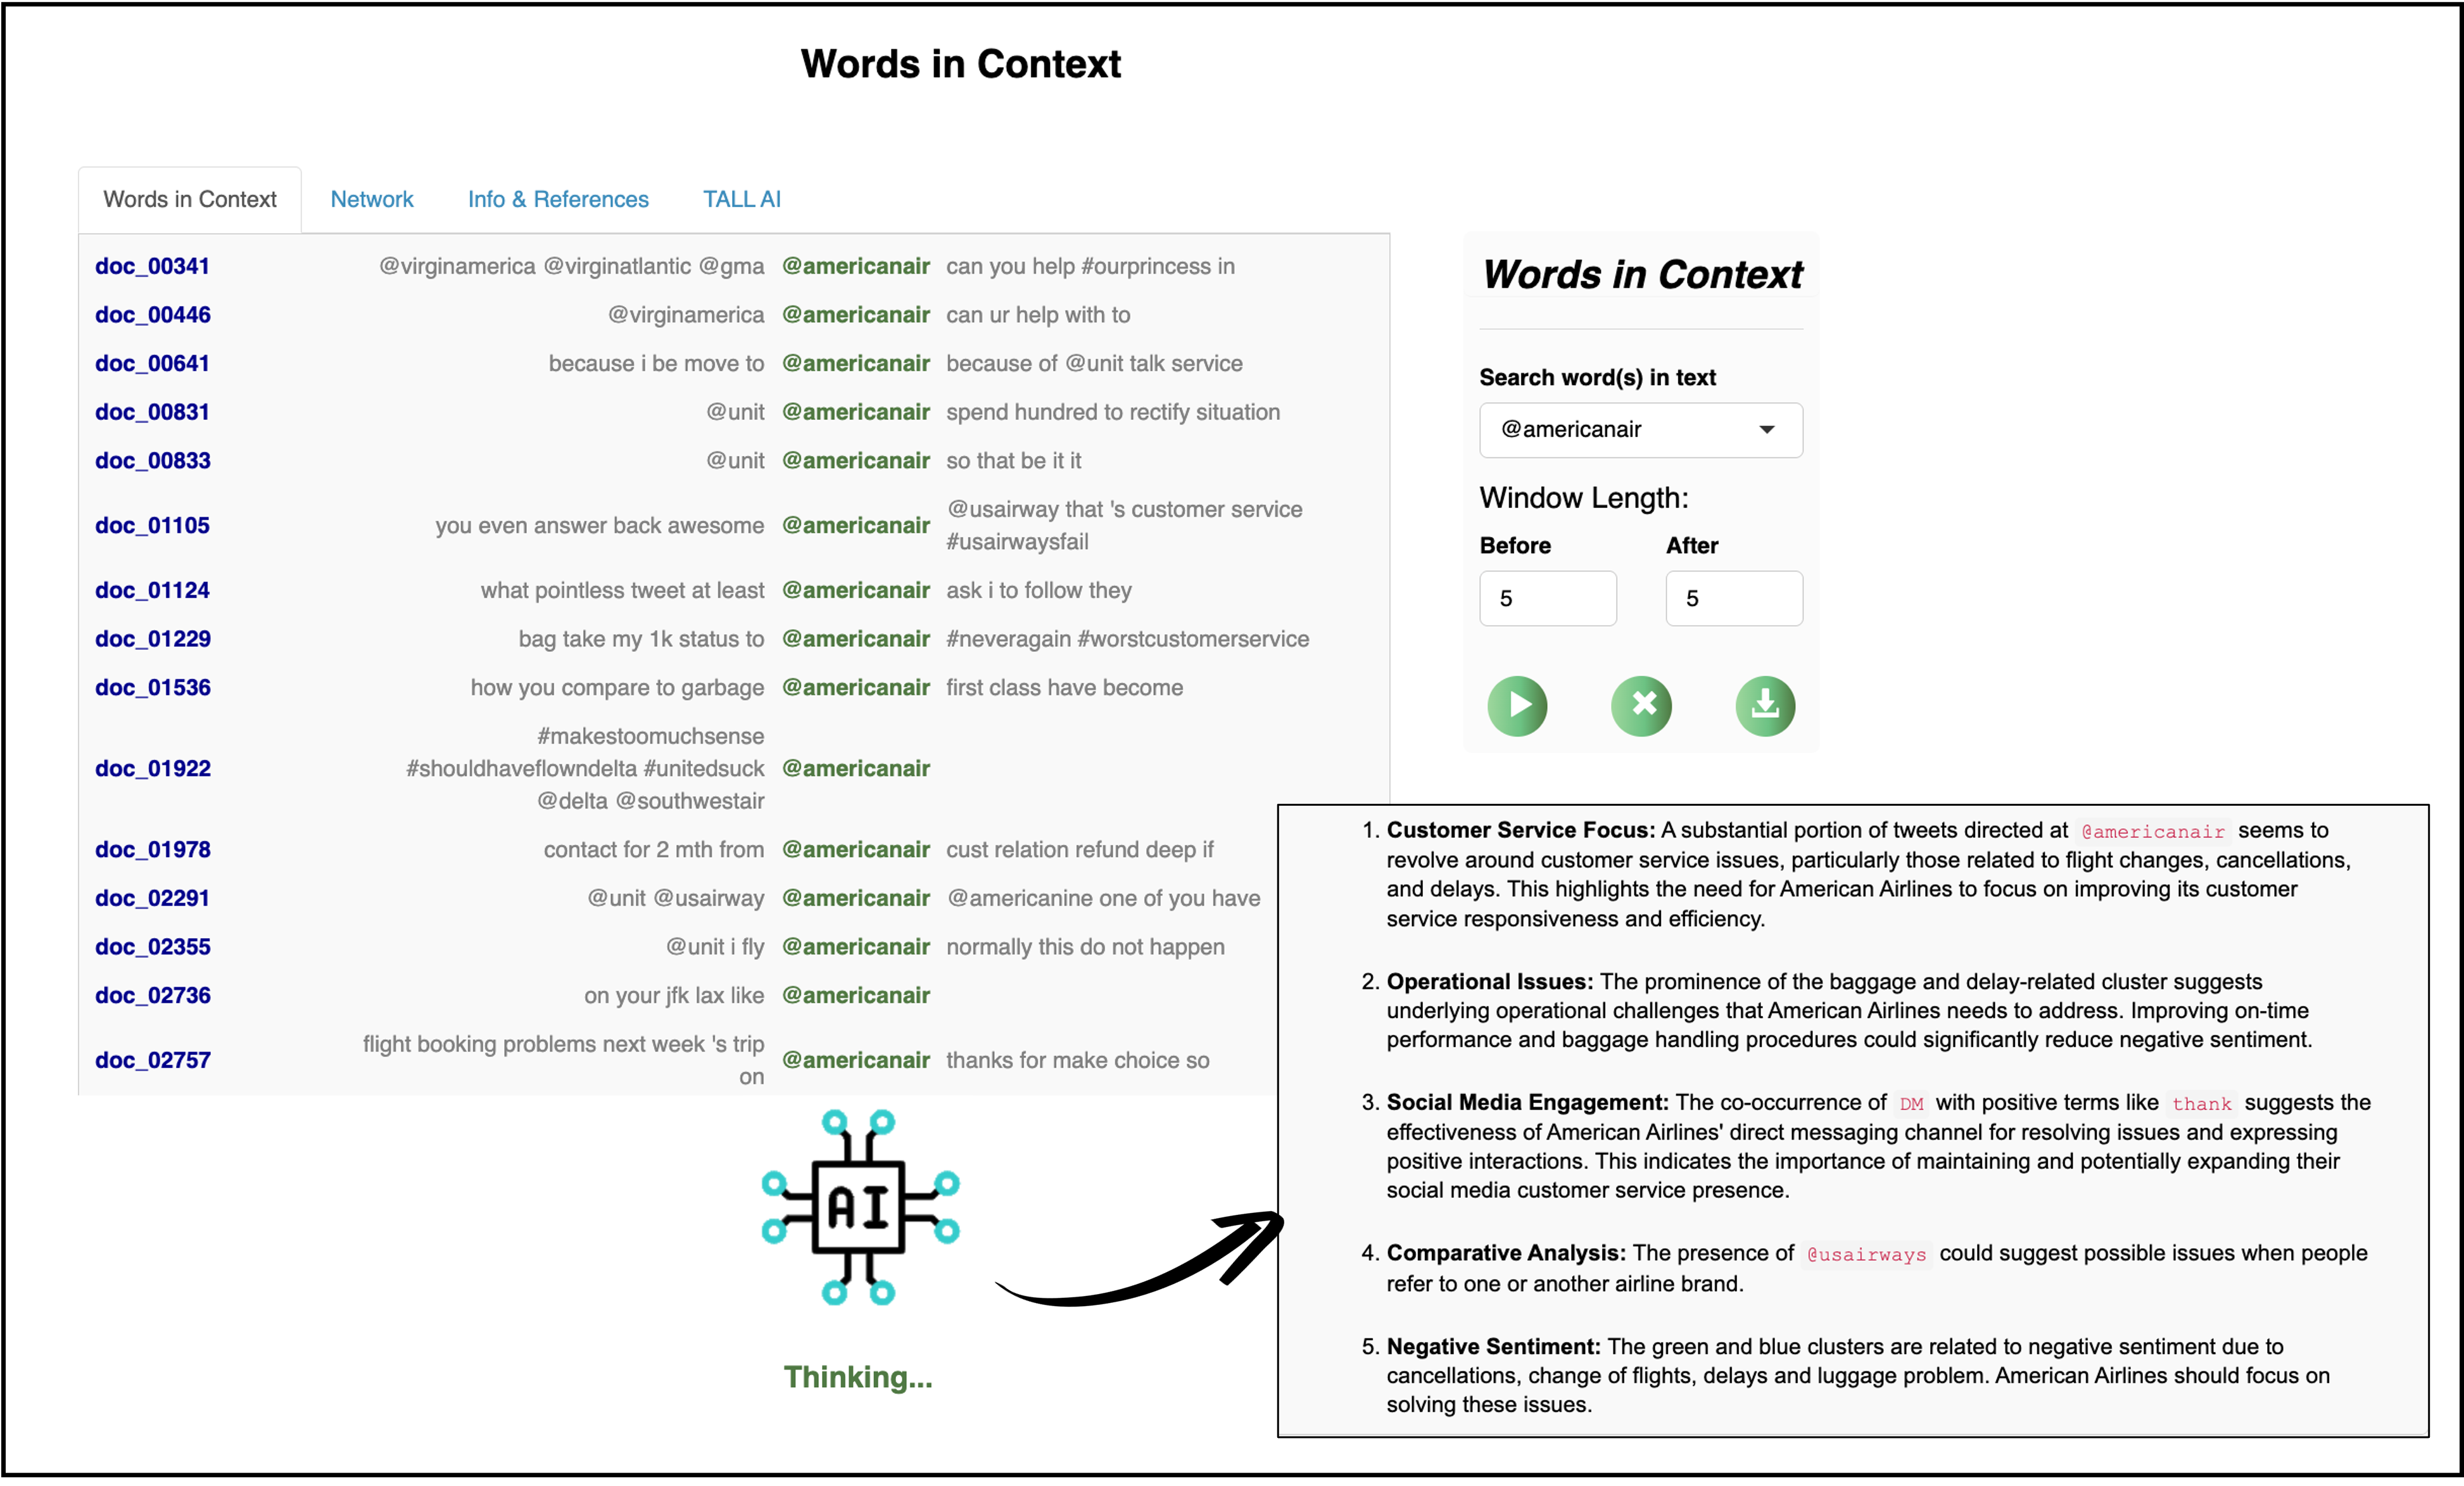
\includegraphics[width=0.865\textwidth]{fig7_context.png}
    \caption{Words in context.}
    \label{fig:context}
\end{figure}

\subsection*{Word-in-Context analysis}
The Word-in-Context module enables detailed examination of how specific terms are employed within their immediate textual environments. This concordance-based approach reveals usage patterns, co-occurring terms, and semantic associations that may not be apparent from frequency counts alone. To illustrate this functionality, the analysis focused on mentions of American Airlines. The concordance view displays each occurrence of ``@AmericanAirlines'' along with its surrounding context, enabling qualitative interpretation of customer interactions with the airline (Fig.~\ref{fig:context}). The TALL AI assistant synthesized these observations into several key insights regarding the role of American Airlines mentions within customer discourse, like Customer Service Focus, Operational Issues, and Social Media Engagement. This analysis demonstrates how the Word-in-Context module facilitates both close reading of textual data and AI-assisted pattern recognition, bridging qualitative and quantitative approaches to corpus analysis.

\subsection*{Polarity detection and sentiment analysis}
At the document level, sentiment analysis was conducted using the Polarity Detection module. Configuration options, accessible via the settings icon, allow users to specify:
\begin{enumerate}
    \item Unit of analysis: Documents (each tweet treated as a separate unit)
    \item Sentiment lexicon: Hu-Liu lexicon \cite{liu04} (selected for this analysis)
    \item Output format: Aggregated distributions and word-level breakdowns
\end{enumerate}

\subsubsection*{I. Overall Sentiment Distribution}
The donut chart visualization (Fig.~\ref{fig:polarity}) provides a high-level overview of sentiment distribution across the corpus:

\begin{itemize}
    \item Neutral sentiment: 48.6\% of tweets
    \item Negative sentiment: 28.03\% (comprising 8.83\% Very Negative and 19.2\% Negative)
    \item Positive sentiment: 23.44\% (comprising 6.54\% Positive and 17.4\% Very Positive)
\end{itemize}

\begin{figure}[!ht]
    \centering
    \fbox{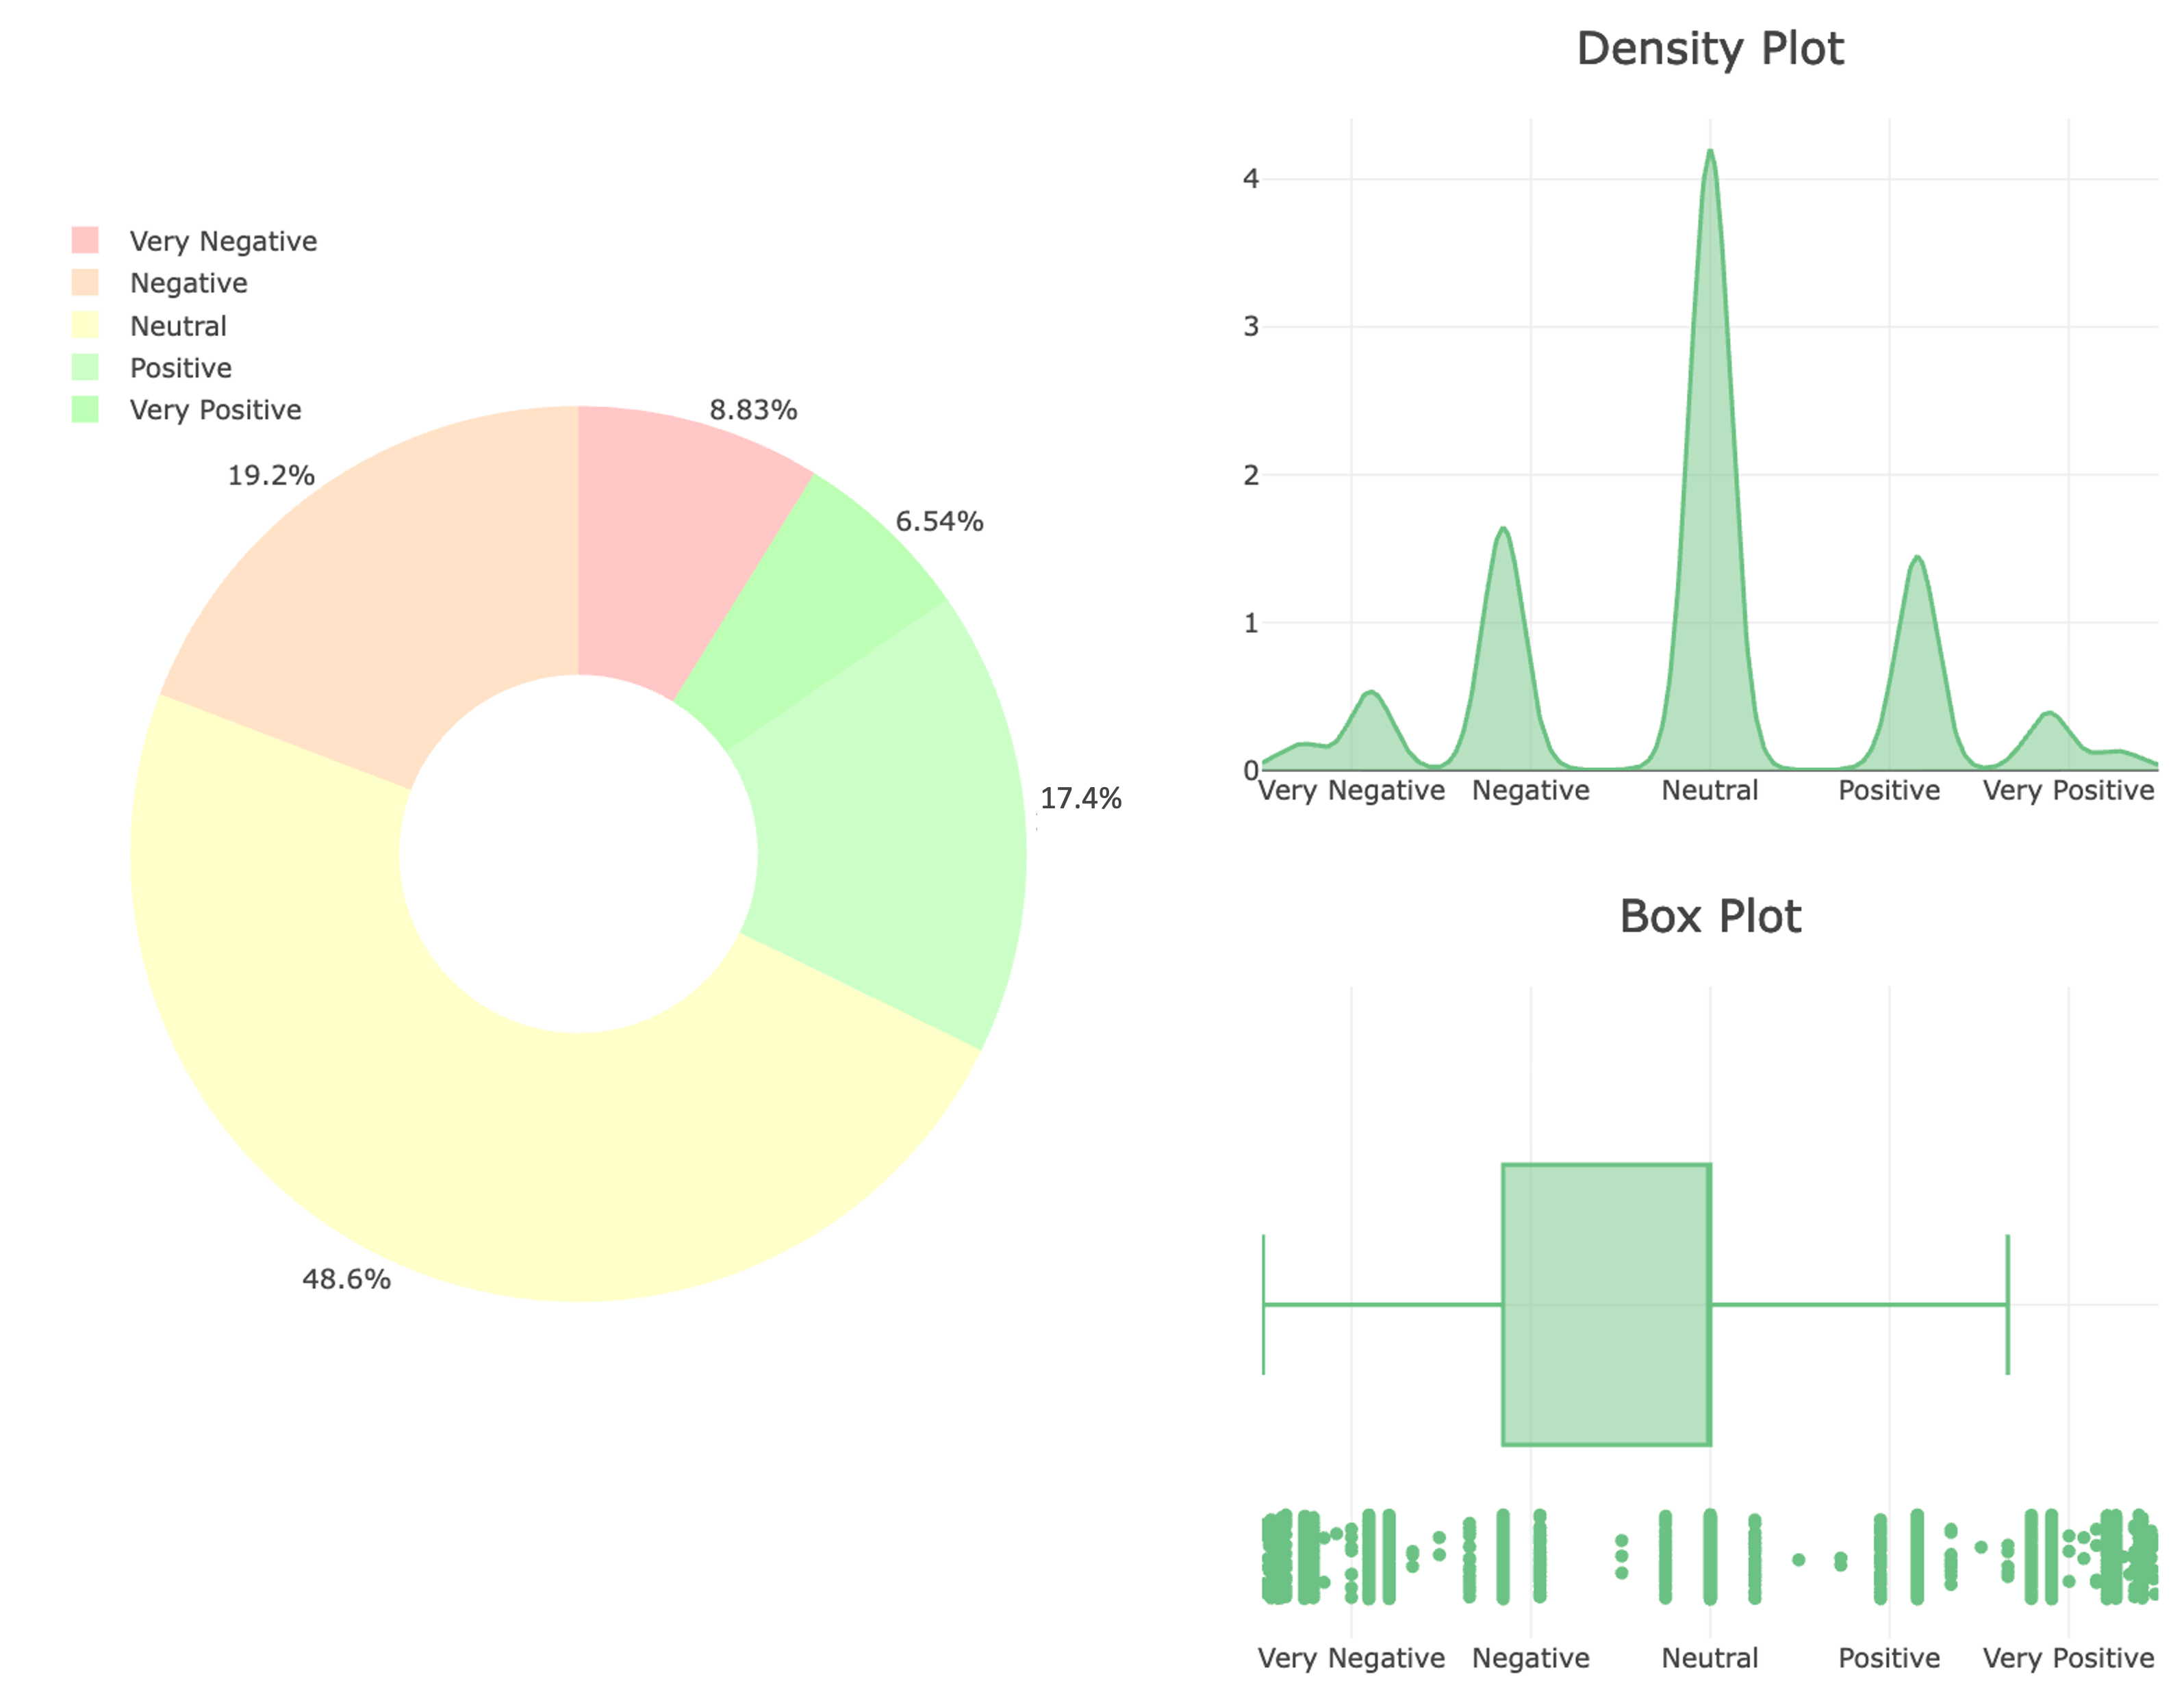
\includegraphics[width=0.9\textwidth]{fig8_polarity.png}}
    \caption{Sentiment distribution (overall polarity).}
    \label{fig:polarity}
\end{figure}

\noindent\textbf{Interpretation}: The predominance of neutral sentiment suggests that a substantial portion of tweets consists of factual inquiries, informational updates, or general mentions lacking strong emotional valence. However, the considerable proportion of negative sentiment (28.03\%) indicates significant customer dissatisfaction during the analyzed period. The bimodal distribution $-$ with neutral sentiment flanked by notable negative and positive segments $-$ reflects typical patterns in service-related social media discourse, where customers are more likely to report problems than routine experiences.

\subsubsection*{II. Top Words by Sentiment Category}
The Top Words panel displays frequency distributions for terms associated with each sentiment category. Analysis of these distributions reveals distinct lexical patterns (Fig.~\ref{fig:topwords}).

\begin{figure}[!ht]
    \centering
    \fbox{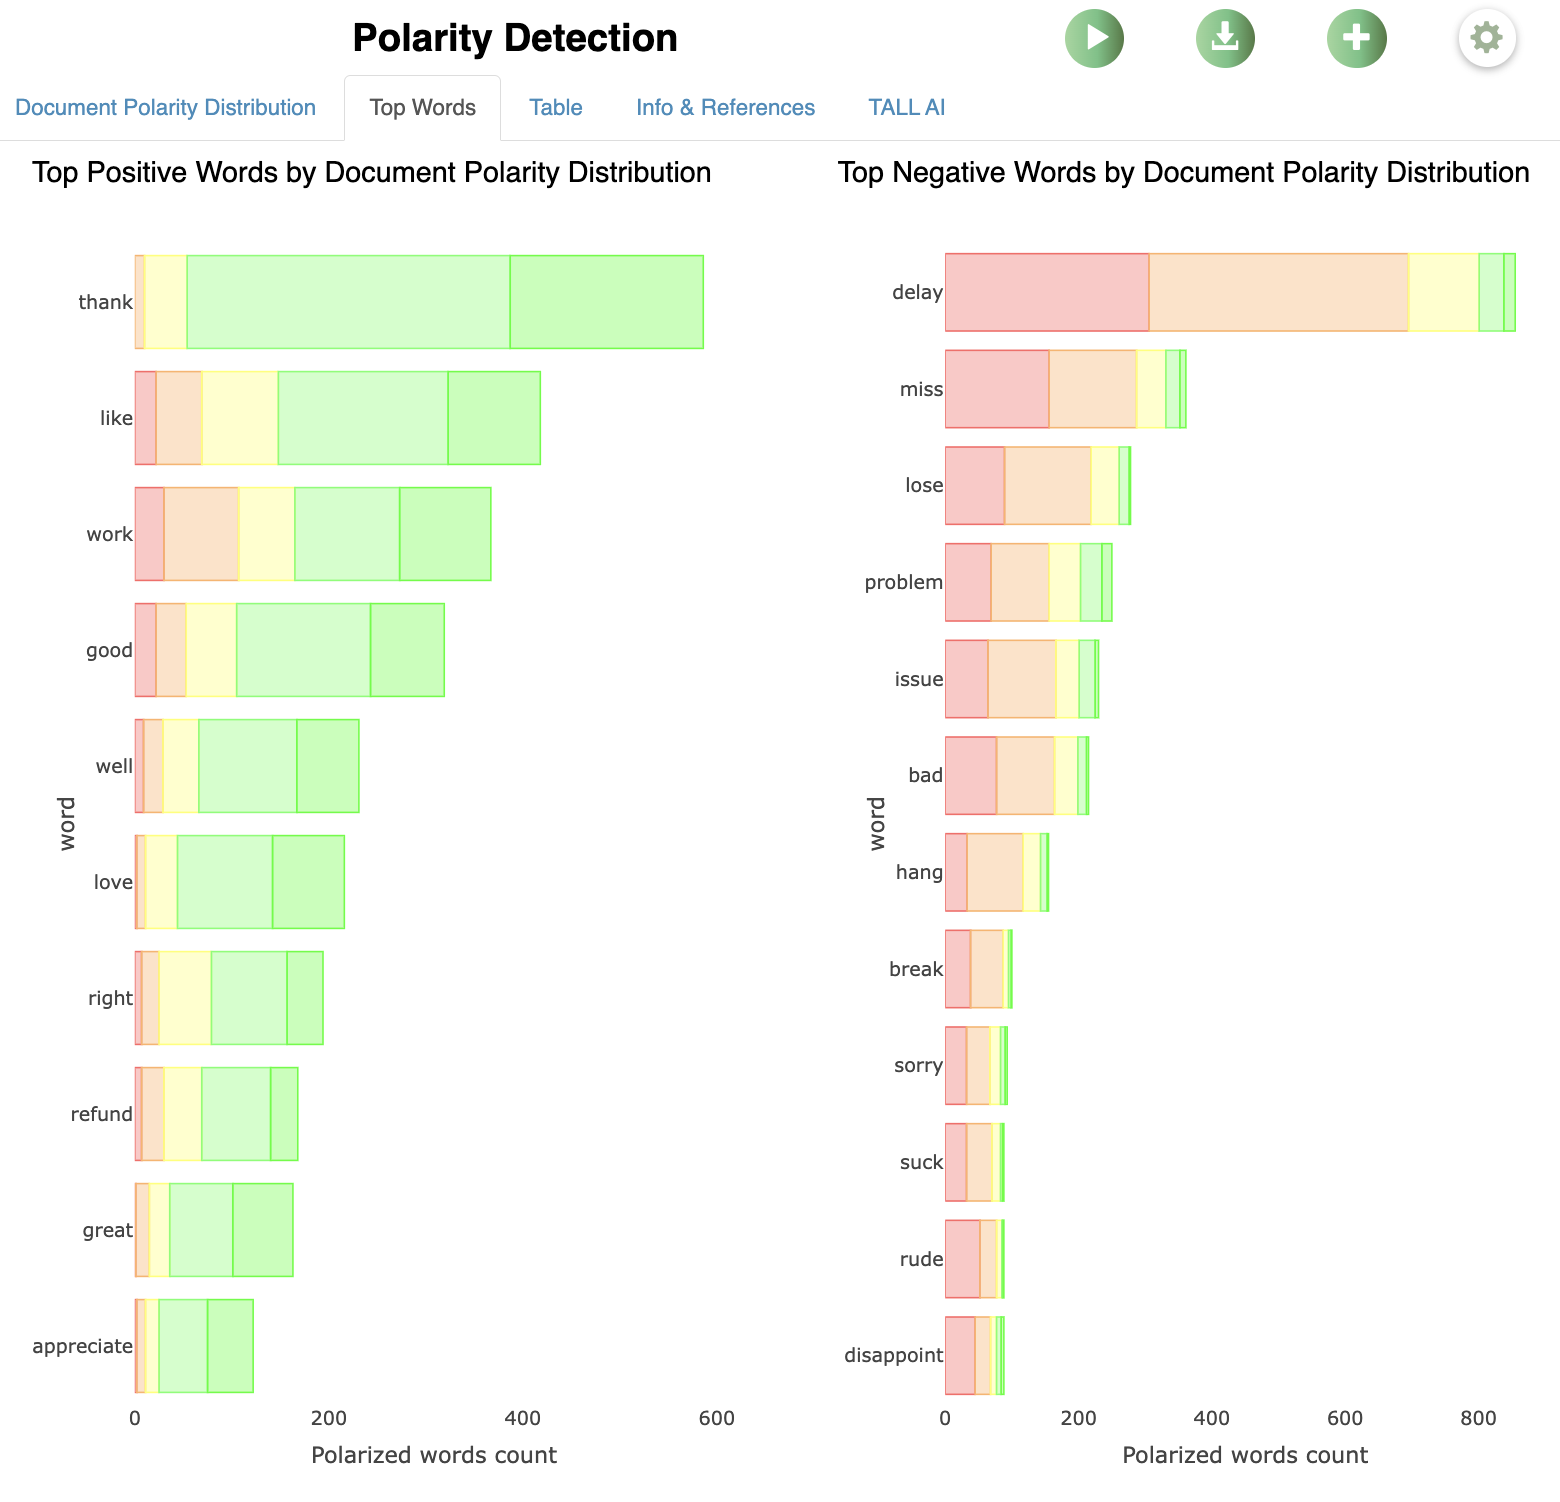
\includegraphics[width=0.8\textwidth]{fig9_topwords.png}}
    \caption{Top word by sentiment category (positive and negative).}
    \label{fig:topwords}
\end{figure}

\vspace{\baselineskip}
\noindent\textit{-- \textbf{Positive Sentiment Words}:}
\begin{enumerate}
    \item \textit{Thank, Good, Great, Love, Appreciate}: Strong indicators of customer satisfaction, with ``thank'' and ``appreciate'' suggesting gratitude for service recovery or exceptional interactions
    \item \textit{Work, Like}: Context-dependent terms appearing across multiple sentiment categories, requiring deeper concordance analysis for precise interpretation
    \item \textit{Refund, Right, Well}: Mixed-valence terms potentially indicating successful issue resolution (``refund'') or service expectations being met (``right,'' ``well'')
\end{enumerate}

\noindent\textit{-- \textbf{Negative Sentiment Words}:}
\begin{enumerate}
    \item \textit{Delay, Miss, Lose, Problem, Issue}: Operationally focused terms highlighting flight disruptions as primary drivers of dissatisfaction
    \item \textit{Bad, Suck, Rude, Disappoint}: Emotionally charged terms expressing strong negative reactions
    \item \textit{Hang, Break}: Potentially referring to communication failures or service breakdowns
    \item \textit{Sorry}: Ambiguous term that may reflect customer frustration or airline attempts at service recovery
\end{enumerate}

\subsubsection*{Key insights and implications}

At the end of the workflow, it is possible to derive interesting insights on the analysed \textit{corpus}:

\begin{enumerate}
    \item \textbf{Confirmation of Sentiment-Specific Vocabulary}: The word distribution analysis validates expected associations between lexical choices and sentiment categories, demonstrating that customer sentiment is reliably encoded in terminology.
    \item \textbf{Operational Issues as Primary Dissatisfiers}: Flight delays, cancellations, and logistical problems dominate negative sentiment, suggesting that operational reliability is critical to customer satisfaction.
    \item \textbf{Opportunities for Service Recovery}: The presence of gratitude-related terms in positive sentiment indicates that effective customer service responses can mitigate dissatisfaction and generate positive outcomes.
    \item \textbf{Contextual Analysis Needed}: Terms like ``work,'' ``like,'' and ``sorry'' require concordance-based examination to understand their role in sentiment expression, illustrating the complementary value of qualitative and quantitative methods.
\end{enumerate}

\begin{thebibliography}{00}

\bibitem{ari25} Aria M. Pre-trained models for TALL [website]. 2025, \url{https://github.com/massimoaria/tall.language.models}

\bibitem{bench25}, Hester J, Vaughan D (2025). bench: High Precision Timing of R Expressions. R package version 1.1.4, \url{https://github.com/r-lib/bench, https://bench.r-lib.org/}

\bibitem{liu04} Hu M, Liu, B. Mining and summarizing customer reviews. In: Proceedings of the tenth ACM SIGKDD international conference on Knowledge discovery and data mining.  New York, NY: ACM; 2004. p. 168–177. \url{https://doi.org/10.1145/1014052.1014073}.

\bibitem{fig15} Figure Eight. Twitter US Airline Sentiment [dataset]. Kaggle Data. 2015. \url{https://www.kaggle.com/datasets/crowdflower/twitter-airline-sentiment}.

\bibitem{ros10} Rose S, Engel D, Cramer N, Cowley W. Automatic keyword extraction from individual documents. In: Berry MW, Kogan J, editors. Text Mining: Applications and Theory. Chichester: Wiley; 2010. p. 1–20. \url{https://doi.org/10.1002/9780470689646.ch1}.

\bibitem{wil16} Wilkinson MD, Dumontier M, Aalbersberg IJ, Appleton G, Axton M, Baak A, et al. The FAIR Guiding Principles for scientific data management and stewardship. Sci Data 2016;3:160018. \url{https://doi.org/10.1038/sdata.2016.18}.

\bibitem{zel17} Zeldes A. The GUM Corpus: Creating Multilayer Resources in the Classroom. Lang Resour Eval 2017;51(3):581–612. \url{http://dx.doi.org/10.1007/s10579-016-9343-x}.

\end{thebibliography}

\end{document}